\documentclass[fleqn,11pt]{article}
\usepackage{bm}
\setlength{\textwidth}{17.5cm}
\setlength{\textheight}{23.2cm}
\setlength{\hoffset}{-2.0cm}
\setlength{\voffset}{-2.5cm}

\usepackage{graphicx}
\usepackage{lastpage}
\usepackage{datetime}
\usepackage{fancyhdr}
\usepackage{amsmath}
\usepackage{float}
\usepackage{hyperref}
\usepackage{color}
\usepackage{xcolor}
\usepackage{listings}
\lstloadlanguages{Matlab,Python,bash,make,C++}
\usepackage{tcolorbox}
\usepackage{svg}
\usepackage{caption}
% \usepackage{subfigure}

\usepackage[utf8]{inputenc}
\usepackage[T1]{fontenc}
\usepackage{textcomp}
\usepackage{gensymb}

\usepackage{multirow}

\include{latex_fei_highlight}

% list and color set.......
%%%%%%%%%%%%%%%%%%%%%%%%%%%%%%%%%%
\usepackage{color}
\usepackage{xcolor}
\usepackage{listings}
\lstloadlanguages{Matlab,Python}
\lstdefinelanguage{fei}
{morekeywords={
20NodeBrick, 27NodeBrick, 8NodeBrick, a0, a1, a2, a3, a4, acceleration, acceleration_file, acceleration_scale_unit, add, algorithm, algorithm
, all
, alpha, and, armstrong_frederick_cr, armstrong_frederick_ha, at, ax, ay, az, bending_Iy, bending_Iz, beta, beta_min, binary
, check, compressive_strength, constant, constitutive, constrain, constraint, contact_plane_vector, control, convergence, cR1, cR2, critical_stress_ratio_M, cross_section, crushing_strength, damping, databasename, define, direction, displacement, displacement_control, displacement_file, displacement_scale_unit, dof, dofs, dofs
, domain, domain
, drained, druckerprager_angle, dynamic, e0, each, eigen, Elastic_Membrane_Plate, elastic_modulus, elastic_modulus_horizontal, elastic_modulus_vertical, element, element_file, else, equal, equaldof, factor, field, filename
, fix, force_file, forces, free, friction_ratio, gamma, Gauss, h_in, help
, host, if, imposed, Imx, Imy, Imz, in, increment, initial_confining_strain, initial_confining_stress, initial_mean_pressure, integration_points, IntegrationRule, integrator, isotropic_hardening_rate, joint_1_offset, joint_2_offset, K_f, K_s, k_x, k_y, k_z, kappa, kd_in, kinematic_hardening_rate, lambda, length, linear
, load, loading, M_in, magnitude, magnitudes, mass, mass_density, master, material, maximum_gap, maximum_number_of_iterations, maximum_strain, maximum_time_step, mean, Membrane_Plate_Fiber, mesh, method, minimum_bulk_modulus, minimum_time_step, model, motion, mx, my, mz, name, new, node, nodes, nodes_file, normal_stiffness, number_of_drm_elements, number_of_drm_nodes, number_of_iterations, number_of_modes, number_of_steps, number_of_subincrements, number_of_times_reaching_maximum_strain, of, output, password, path_series, path_time_series, penalty, penalty_for_applying_generalized_displacement, point, points, poisson_ratio, poisson_ratio_h_h, poisson_ratio_h_v, porosity, port, pressure, pressure_reference_p0, print, R0, reduction, reference_void_ratio, remove, response, restore, rho_f, rho_s, rx, ry, rz
, sanisand2004_A0, sanisand2004_c, sanisand2004_ch, sanisand2004_cz, sanisand2004_ec_ref, sanisand2004_G0, sanisand2004_h0, sanisand2004_lambda_c, sanisand2004_m, sanisand2004_Mc, sanisand2004_nb, sanisand2004_nd, sanisand2004_p_cut, sanisand2004_Pat, sanisand2004_xi, sanisand2004_z_max, sanisand2008_A0, sanisand2008_alpha_cc, sanisand2008_c, sanisand2008_ch, sanisand2008_cz, sanisand2008_ec_ref, sanisand2008_G0, sanisand2008_h0, sanisand2008_K0, sanisand2008_k_c, sanisand2008_lambda, sanisand2008_m, sanisand2008_nb, sanisand2008_nd, sanisand2008_p0, sanisand2008_p_in, sanisand2008_p_r, sanisand2008_Pat, sanisand2008_rho_c, sanisand2008_theta_c, sanisand2008_X, sanisand2008_xi, sanisand2008_z_max, save, scale_factor, section, self_weight, series_file, shear, shear_modulus, shear_modulus_h_v, simple, simulate, single, slave, socket, solver, stage, state, static, steps, stiffness, stiffness_to_use, strain, strain_at_compressive_strength, strain_at_crushing_strength, strain_hardening_ratio, strain_increment_size, stress, surface, tangential_stiffness, tensile_strength, tension_softening_stiffness, test, testing, thickness, time_step, to, tolerance_1, tolerance_2, torsion_Jx, triaxial, type, undrained, unit, use, username, using, ux, uy, uz, value, variable_node_brick_8_to_27, velocity_file, velocity_scale_unit, viscoelastic_modulus, von_mises_radius, while, whos
, with, x_max, x_min, xi_in, xz_plane_vector, y_max, y_min, yield_strength, z_max, z_min},
morekeywords={[2] 20NodeBrick, 20NodeBrick_elastic, 20NodeBrick_upU, 27NodeBrick, 27NodeBrick_elastic, 27NodeBrickLT, 3NodeShell_ANDES, 4NodeShell_ANDES, 4NodeShell_MITC4, 4NodeShell_NewMITC4, 8NodeBrick, 8NodeBrick_elastic, 8NodeBrick_up, 8NodeBrick_upU, 8NodeBrickLT, beam_9dof_elastic, beam_displacement_based, beam_elastic, beam_elastic_lumped_mass, camclay, camclay_accelerated, Caughey3rd, Caughey4th, contact, DOFTYPE, druckerprager_isotropic_hardening, druckerprager_isotropic_hardening_accelerated, druckerprager_kinematic_hardening, druckerprager_kinematic_hardening_accelerated, druckerprager_perfectly_plastic, druckerprager_perfectly_plastic_accelerated, Energy_Increment, F_fluid_x, F_fluid_y, F_fluid_z, FORCETYPE, from_reactions, Fx, Fy, Fz, Hilber_Hughes_Taylor, linear, linear_elastic_crossanisotropic, linear_elastic_isotropic_3d, Modified_Newton, Mx, My, mysql, Mz, New_PisanoLT, Newmark, Newton, Norm_Displacement_Increment, Norm_Unbalance, path_series, path_time_series, pisano, pisanoLT, ProfileSPD, Rayleigh, sanisand2004, sanisand2008, static, transient, truss, UMFPack, uniaxial_concrete02, uniaxial_elastic, uniaxial_steel01, uniaxial_steel02, variable transient, vonmises_isotropic_hardening, vonmises_isotropic_hardening_accelerated, vonmises_kinematic_hardening, vonmises_kinematic_hardening_accelerated, vonmises_linear_kinematic_hardening, vonmises_linear_kinematic_hardening_accelerated, vonmises_perfectly_plastic, vonmises_perfectly_plastic_accelerated, vonmises_perfectly_plastic_LT, With_no_convergence_check,
elastic_modulus_1atm,m_in,n_in,a_in,eplcum_cr_in},
sensitive=true,
morecomment=[l]{//},
morestring=[b]",
}

\definecolor{dkgreen}{rgb}{0,0.6,0}
\definecolor{gray}{rgb}{0.5,0.5,0.5}
\definecolor{mauve}{rgb}{0.58,0,0.82}
\definecolor{ltgray}{rgb}{0.98,0.98,0.98}
\definecolor{grayish}{rgb}{0.85, 0.85, 0.85}
\lstset{language=fei, 
  frame=single,
  backgroundcolor=\color{ltgray},
  aboveskip=3mm,
  belowskip=3mm,
  showstringspaces=false,
  columns=flexible,
  basicstyle={\small\ttfamily},
  numberstyle=\tiny\color{black},
  keywordstyle=\color{blue},
  commentstyle=\color{gray},
  stringstyle=\color{mauve},
  breaklines=true,
  numbers=left,
  breakatwhitespace=true,
  tabsize=3,
  %rulecolor=\color{mauve},
}

% list and color set.......
%%%%%%%%%%%%%%%%%%%%%%%%%%%%%%%%%%
\usepackage{color}
\usepackage{xcolor}
\usepackage{listings}


\pagestyle{fancy}

\def\today
{\number\day.\space \ifcase\month\or
January\or
February\or
March\or
April\or
May\or
June\or
July\or
August\or
September\or
October\or
November\or
December\fi,\space
\number\year}

%%%%
\newcount\hh
\newcount\mm
\mm=\time
\hh=\time
\divide\hh by 60
\divide\mm by 60
\multiply\mm by 60
\mm=-\mm
\advance\mm by \time
\def\hhmm{\number\hh:\ifnum\mm<10{}0\fi\number\mm}

%%%%%
\lhead{\small \it Yuan Feng}
\chead{\small Education Examples for Constitutive Material Behavior}
\rhead{\small \it \thepage{} of \pageref{LastPage} }
%
\lfoot{\small \it Univ. of California, Davis}
\rfoot{\small \it \today, \hhmm}
\cfoot{\small }
\addtolength{\headheight}{14pt}


\title{Education Examples for Constitutive Material Behavior}
\author{Yuan Feng}
\begin{document}
\thispagestyle{fancy}
\maketitle
\tableofcontents

%%%%%%%%%%%%%%%%%%%%%%%%%%%%%%%%%%%%%%%%%%%%%%%%%%%%%%%%%%%%%%%%%
%%%%%%%%%%%%%%%%%%%%%%%%%%%%%%%%%%%%%%%%%%%%%%%%%%%%%%%%%%%%%%%%%
%%%%%%%%%%%%%%%%%%%%%%%%%%%%%%%%%%%%%%%%%%%%%%%%%%%%%%%%%%%%%%%%%
\newpage
\section{Chapter Summary and Highlights}

In the Chapter, the mechanical behaviors of elastoplastic materials
is tested. The purpose is to simulate the simplest material points
or the simplest solid brick for the sake of education. 

Section.\ref{section_elastic_constitutive_example} and 
Section.\ref{section_elastoplastic_constitutive_example} are testing
one material point directly. 

Section.\ref{section_elastic_brick_example} and 
Section.\ref{section_elastoplastic_brick_example} are testing the 
material (Gauss Points) through the 8-node solid brick element. 

Distinct yield surfaces are tested, including von-Mises and 
Drucker-Prager yield surfaces with associative and 
non-associative plastic flow. 

Likewise, various hardening rules are simulated, including 
isotropic hardening, kinematic hardening, 
Armstrong-Frederick hardening, and multi-yield-surface hardening.

%%%%%%%%%%%%%%%%%%%%%%%%%%%%%%%%%%%%%%%%%%%%%%%%%%%%%%%%%%%%%%%%%
%%%%%%%%%%%%%%%%%%%%%%%%%%%%%%%%%%%%%%%%%%%%%%%%%%%%%%%%%%%%%%%%%
%%%%%%%%%%%%%%%%%%%%%%%%%%%%%%%%%%%%%%%%%%%%%%%%%%%%%%%%%%%%%%%%%



%%%%%%%%%%%%%%%%%%%%%%%%%%%%%%%%%%%%%%%%%%%%%%%%%%%%%%%%%%%%%%%%%%%%%%%%%%%%
%%%%%%%%%%%%%%%%%%%%%%%%%%%%%%%%%%%%%%%%%%%%%%%%%%%%%%%%%%%%%%%%%%%%%%%%%%%%
%%%%%%%%%%%%%%%%%%%%%%%%%%%%%%%%%%%%%%%%%%%%%%%%%%%%%%%%%%%%%%%%%%%%%%%%%%%%
%%%%%%%%%%%%%%%%%%%%%%%%%%%%%%%%%%%%%%%%%%%%%%%%%%%%%%%%%%%%%%%%%%%%%%%%%%%%
%%%%%%%%%%%%%%%%%%%%%%%%%%%%%%%%%%%%%%%%%%%%%%%%%%%%%%%%%%%%%%%%%%%%%%%%%%%%
%%%%%%%%%%%%%%%%%%%%%%%%%%%%%%%%%%%%%%%%%%%%%%%%%%%%%%%%%%%%%%%%%%%%%%%%%%%%
\newpage
\section{Elastic Solid Constitutive Examples}
\label{section_elastic_constitutive_example}
%%%%%%%%%%%%%%%%%%%%%%%%%%%%%%%%%%%%%%%%%%%%%%%%%%%%%%%%%%%%%%%%%%%%%%%%%%%%
\subsection{Linear Elastic Constitutive Examples}

%%%%%%%%%%%%%%%%%%%%%%%%%%%%%%%%%%%%%%%%%%%%%%%%%%%%%%%%%%%%%%%%%%%%%%%%%%%%
\paragraph{Pure Shear, Monotonic Loading} ~ 

Material Parameters:
\lstinputlisting{../fei_examples/linear_elastic/1pure_shear_mono_loading/main.fei}

Material Response:
\begin{figure}[H]
\begin{center}
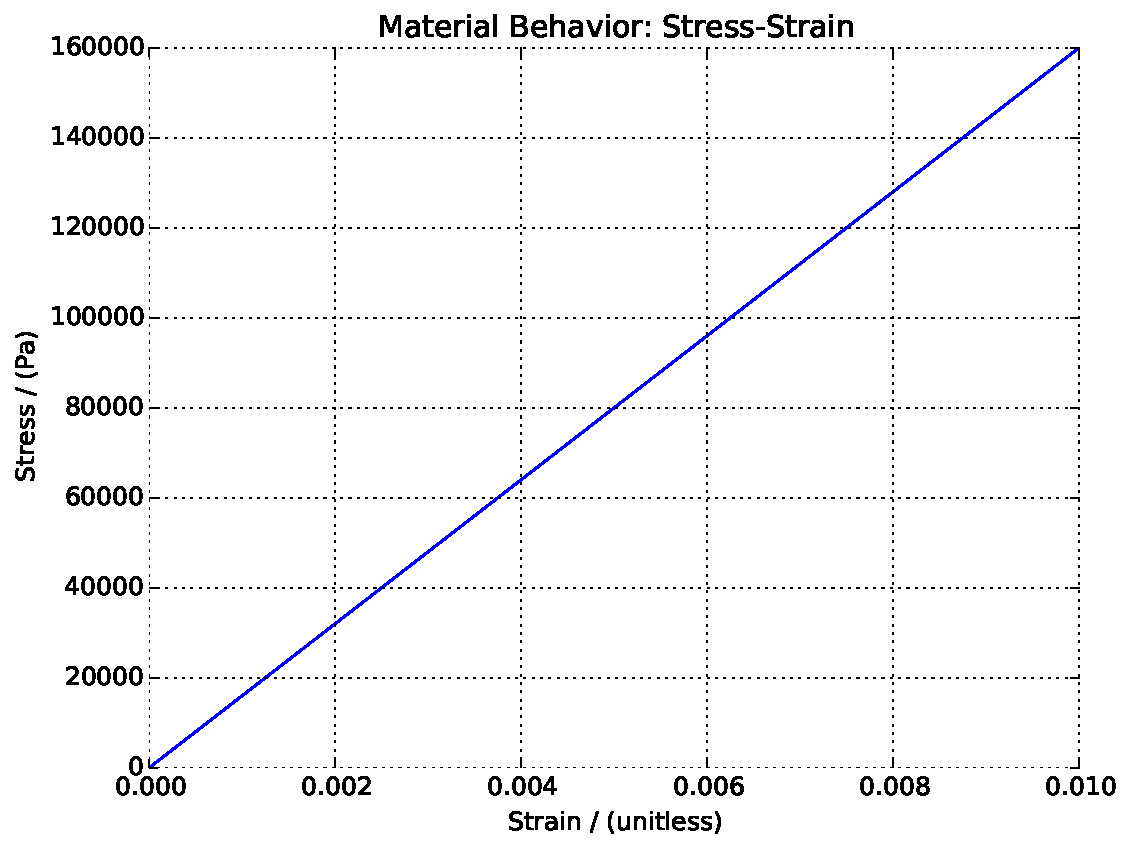
\includegraphics[width=12cm]{../fei_examples/linear_elastic/1pure_shear_mono_loading/result.pdf}
\caption{
\label{constitutive_linear_elastic Pure Shear Monotomic Loadin}
Linear Elastic Pure Shear Monotomic Loading}
\end{center}
\end{figure}

The fei files for this example are available \href{https://github.com/yuan-energy/education_examples/tree/master/fei_examples/linear_elastic/1pure_shear_mono_loading}{here}.

%%%%%%%%%%%%%%%%%%%%%%%%%%%%%%%%%%%%%%%%%%%%%%%%%%%%%%%%%%%%%%%%%%%%%%%%%%%%
\newpage
\paragraph{Pure Shear, Cyclic Loading} ~ 

Material Parameters:
\lstinputlisting{../fei_examples/linear_elastic/2pure_shear_cyclic_loading/main.fei}

Material Response:
\begin{figure}[H]
\begin{center}
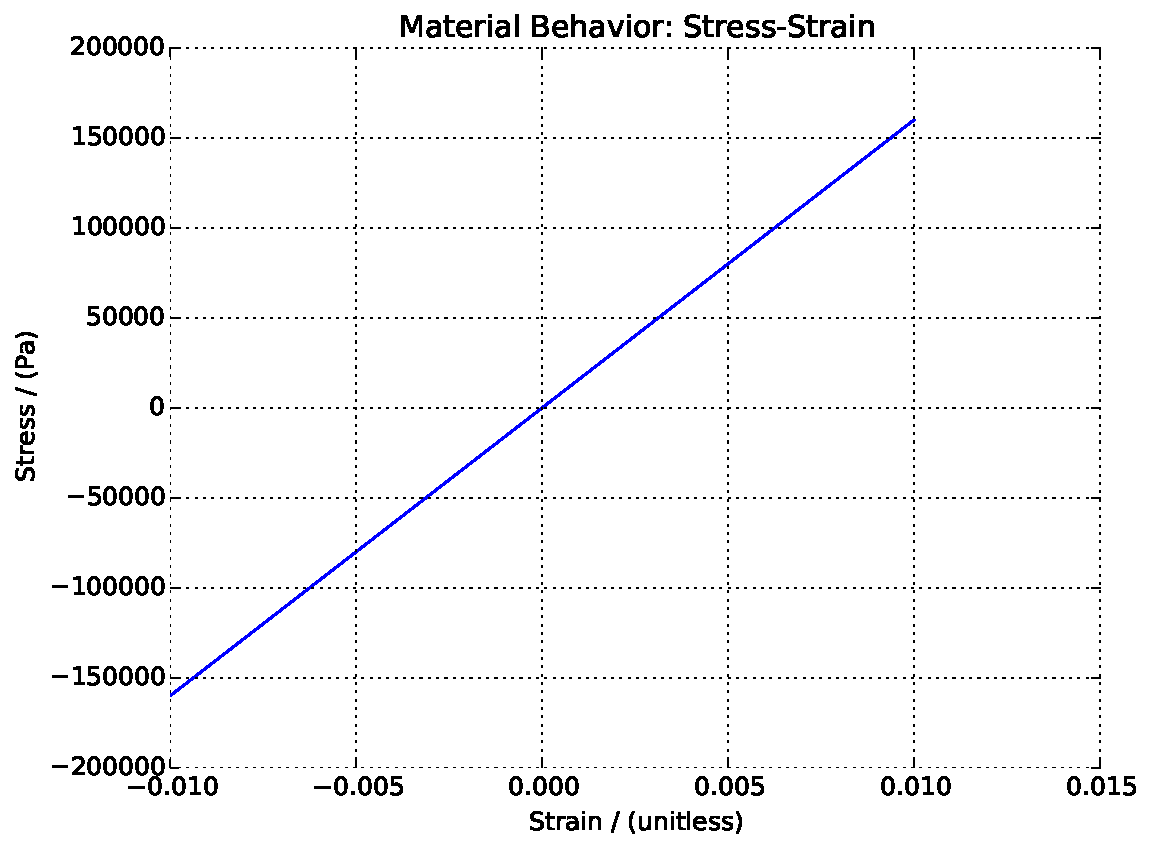
\includegraphics[width=12cm]{../fei_examples/linear_elastic/2pure_shear_cyclic_loading/result.pdf}
\caption{
\label{Linear Elastic Solid_Pure Shear Cyclic Loadin}
Linear Elastic Pure Shear Cyclic Loading}
\end{center}
\end{figure}

The fei files for this example are available \href{https://github.com/yuan-energy/education_examples/tree/master/fei_examples/linear_elastic/2pure_shear_cyclic_loading}{here}.

%%%%%%%%%%%%%%%%%%%%%%%%%%%%%%%%%%%%%%%%%%%%%%%%%%%%%%%%%%%%%%%%%%%%%%%%%%%%
\newpage
\paragraph{Uniaxial Strain, Monotonic Loading} ~ 

Material Parameters:
\lstinputlisting{../fei_examples/linear_elastic/3uniaxial_strain_mono_loading/main.fei}

Material Response:
\begin{figure}[H]
\begin{center}
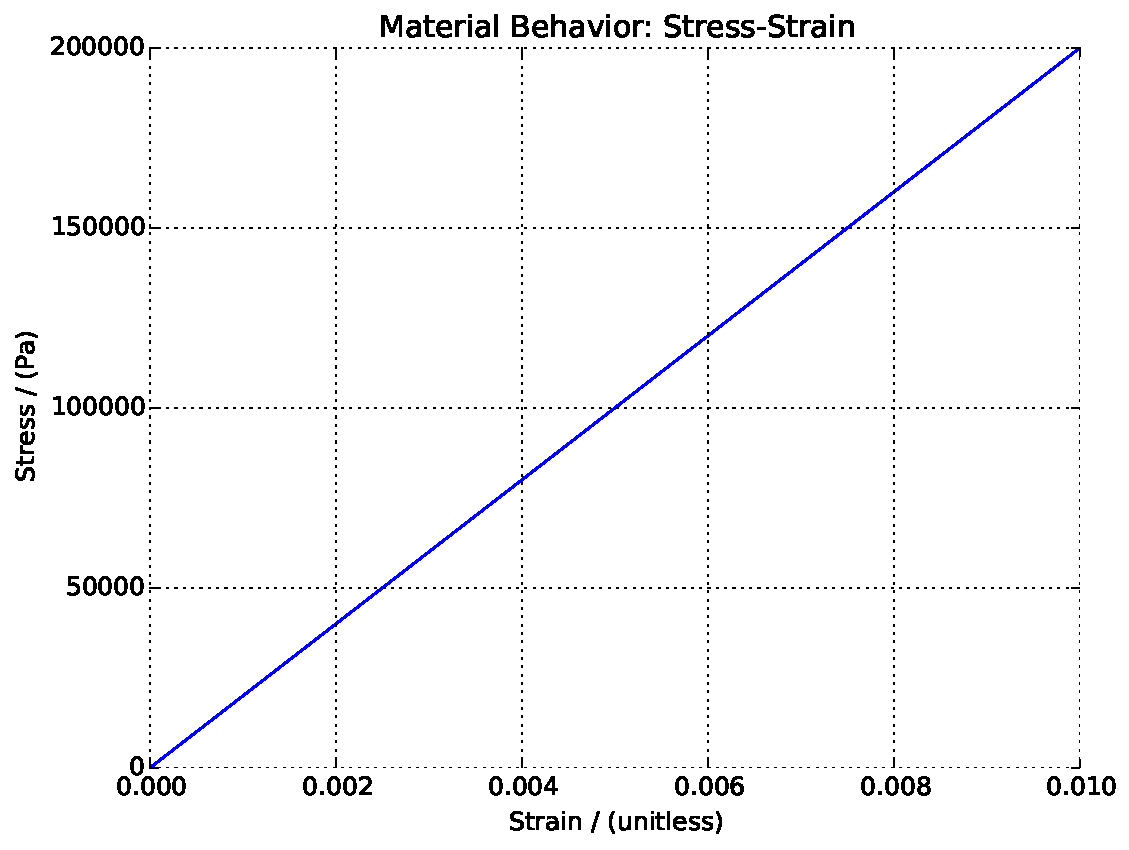
\includegraphics[width=12cm]{../fei_examples/linear_elastic/3uniaxial_strain_mono_loading/result.pdf}
\caption{
\label{Linear Elastic Uniaxial Monotonic Loading}
Linear Elastic Uniaxial Monotonic Loading}
\end{center}
\end{figure}

The fei files for this example are available \href{https://github.com/yuan-energy/education_examples/tree/master/fei_examples/linear_elastic/3uniaxial_strain_mono_loading}{here}.

%%%%%%%%%%%%%%%%%%%%%%%%%%%%%%%%%%%%%%%%%%%%%%%%%%%%%%%%%%%%%%%%%%%%%%%%%%%%
\newpage
\paragraph{Uniaxial Strain, Cyclic Loading} ~

Material Parameters:
\lstinputlisting{../fei_examples/linear_elastic/2pure_shear_cyclic_loading/main.fei}

Material Response:
\begin{figure}[H]
\begin{center}
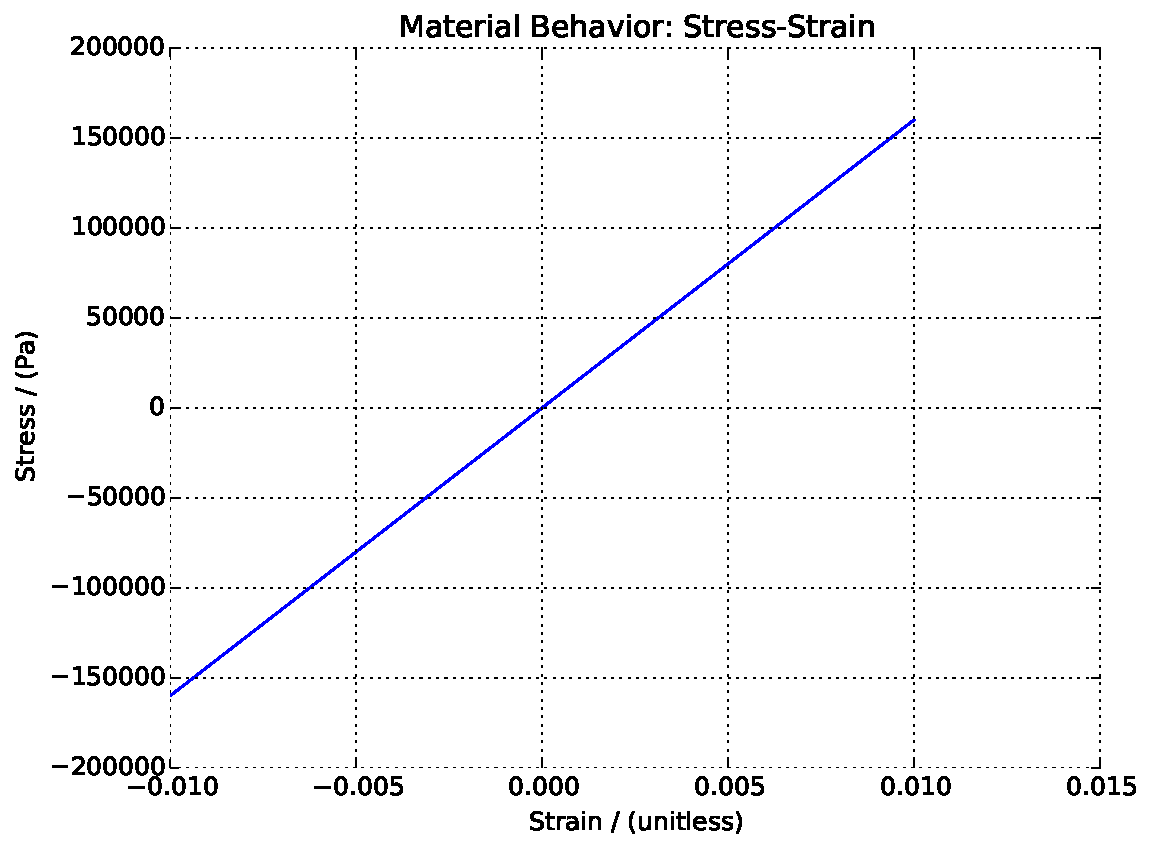
\includegraphics[width=12cm]{../fei_examples/linear_elastic/2pure_shear_cyclic_loading/result.pdf}
\caption{
\label{Linear Elastic Uniaxial Cyclic Loading}
Linear Elastic Uniaxial Cyclic Loading}
\end{center}
\end{figure}

The fei files for this example are available \href{https://github.com/yuan-energy/education_examples/tree/master/fei_examples/linear_elastic/4uniaxial_strain_cyclic_loading}{here}.

%%%%%%%%%%%%%%%%%%%%%%%%%%%%%%%%%%%%%%%%%%%%%%%%%%%%%%%%%%%%%%%%%%%%%%%%%%%%
\newpage
\subsection{Nonlinear Elastic Constitutive Examples}

%%%%%%%%%%%%%%%%%%%%%%%%%%%%%%%%%%%%%%%%%%%%%%%%%%%%%%%%%%%%%%%%%%%%%%%%%%%%
\paragraph{Triaxial Uniform Pressure, Monotonic Loading} ~

The Duncan-Chang nonlinear elastic materials:
\begin{equation}
  E = E_0 - \kappa * p
\end{equation}
where $E_0$ is the initial elastic modulus, parameter $\kappa$ is a material constant, and $p$ is the pressure $p$, where the compresssive pressure is defined as positive in Real ESSI.

Material Parameters:
\lstinputlisting{../fei_examples/duncan_chang_nonlinear_elasticity/1triaxial_uniform_mono_loading/main.fei}

Material Response:
\begin{figure}[H]
\begin{center}
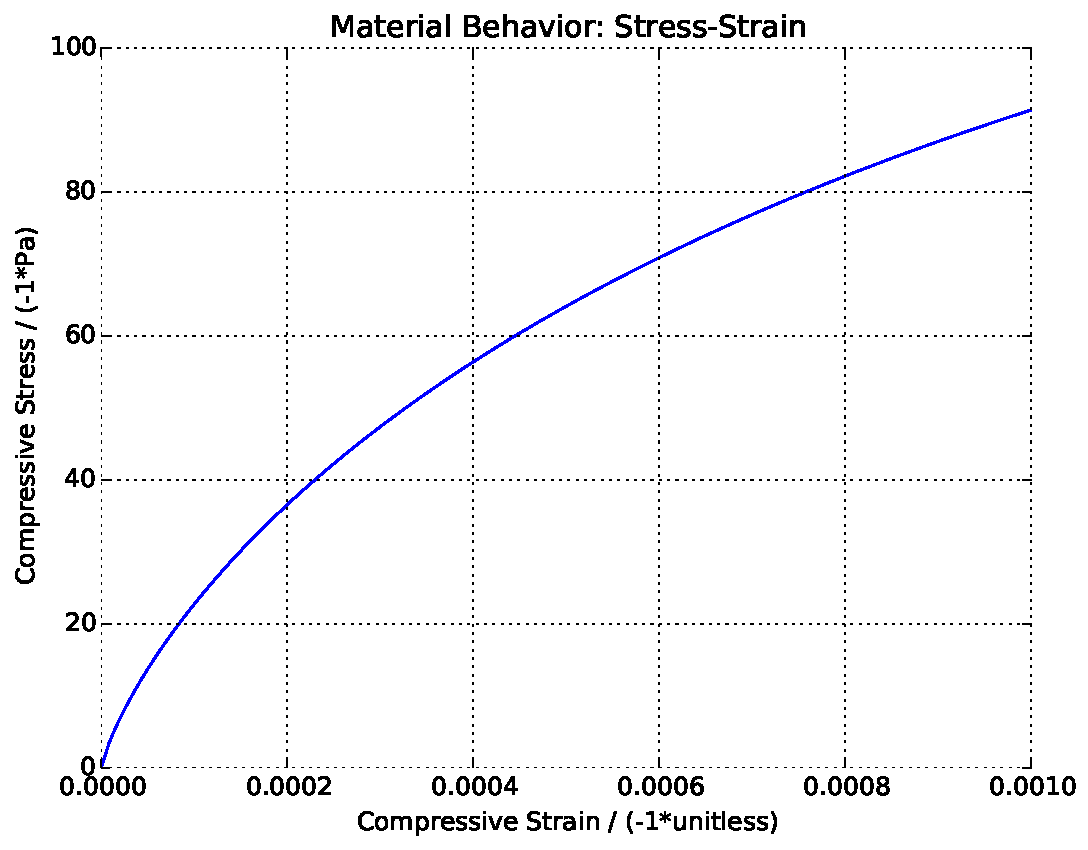
\includegraphics[width=12cm]{../fei_examples/duncan_chang_nonlinear_elasticity/1triaxial_uniform_mono_loading/result.pdf}
\caption{
\label{Res_triaxial_nonlinear_elastic_mono}
Results of Duncan-Chang Nonlinear Elastic Monotonic Loading}
\end{center}
\end{figure}

The fei files for this example are available \href{https://github.com/yuan-energy/education_examples/tree/master/fei_examples/duncan_chang_nonlinear_elasticity/1triaxial_uniform_mono_loading}{here}.

%%%%%%%%%%%%%%%%%%%%%%%%%%%%%%%%%%%%%%%%%%%%%%%%%%%%%%%%%%%%%%%%%%%%%%%%%%%%
\newpage
\subsection{Nonlinear Elastic Constitutive Examples}

%%%%%%%%%%%%%%%%%%%%%%%%%%%%%%%%%%%%%%%%%%%%%%%%%%%%%%%%%%%%%%%%%%%%%%%%%%%%
\paragraph{Triaxial Uniform Pressure, Cyclic Loading} ~

Material Parameters:
\lstinputlisting{../fei_examples/duncan_chang_nonlinear_elasticity/2triaxial_uniform_cyclic_loading/main.fei}

Material Response:
\begin{figure}[H]
\begin{center}
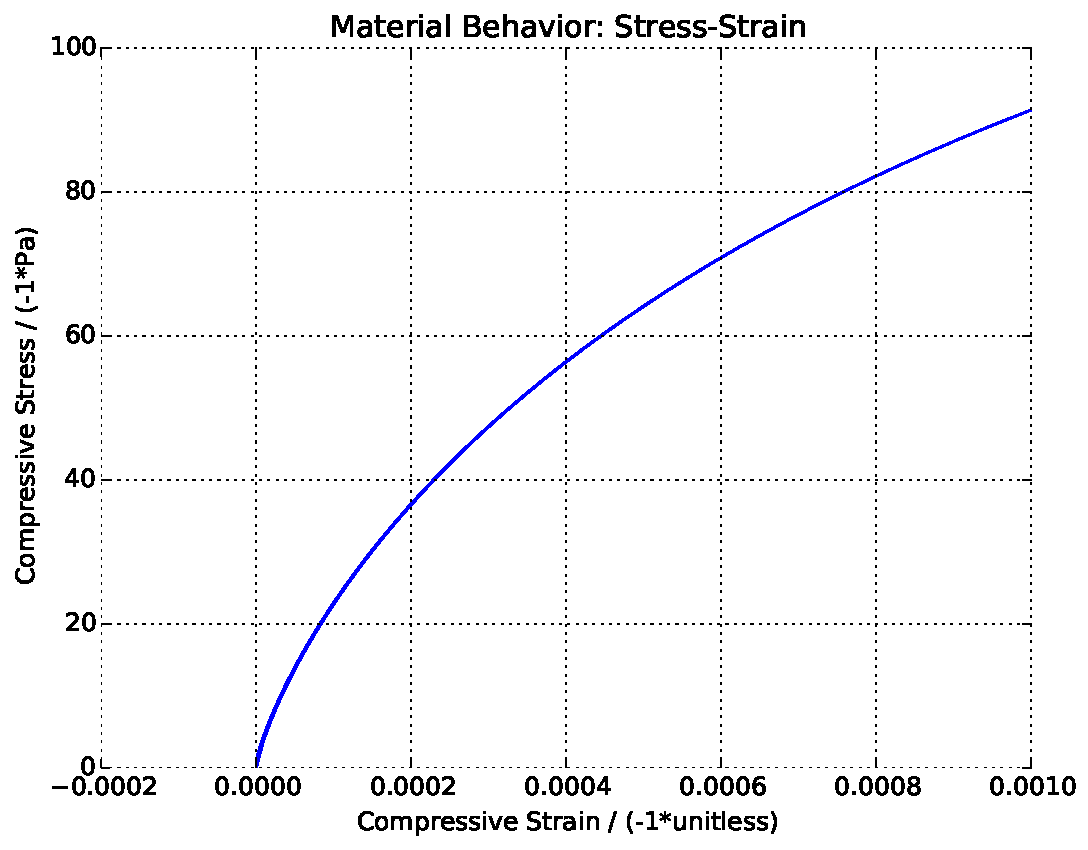
\includegraphics[width=12cm]{../fei_examples/duncan_chang_nonlinear_elasticity/2triaxial_uniform_cyclic_loading/result.pdf}
\caption{
\label{Res_triaxial_nonlinear_elastic_cyclic}
Results of Duncan-Chang Nonlinear Elastic Cyclic Loading}
\end{center}
\end{figure}

The fei files for this example are available \href{https://github.com/yuan-energy/education_examples/tree/master/fei_examples/duncan_chang_nonlinear_elasticity/2triaxial_uniform_cyclic_loading}{here}.













%%%%%%%%%%%%%%%%%%%%%%%%%%%%%%%%%%%%%%%%%%%%%%%%%%%%%%%%%%%%%%%%%%%%%%%%%%%%
%%%%%%%%%%%%%%%%%%%%%%%%%%%%%%%%%%%%%%%%%%%%%%%%%%%%%%%%%%%%%%%%%%%%%%%%%%%%
%%%%%%%%%%%%%%%%%%%%%%%%%%%%%%%%%%%%%%%%%%%%%%%%%%%%%%%%%%%%%%%%%%%%%%%%%%%%
%%%%%%%%%%%%%%%%%%%%%%%%%%%%%%%%%%%%%%%%%%%%%%%%%%%%%%%%%%%%%%%%%%%%%%%%%%%%
%%%%%%%%%%%%%%%%%%%%%%%%%%%%%%%%%%%%%%%%%%%%%%%%%%%%%%%%%%%%%%%%%%%%%%%%%%%%
%%%%%%%%%%%%%%%%%%%%%%%%%%%%%%%%%%%%%%%%%%%%%%%%%%%%%%%%%%%%%%%%%%%%%%%%%%%%
\newpage
\section{Elastic Plastic Solid Constitutive Examples}
\label{section_elastoplastic_constitutive_example}
%%%%%%%%%%%%%%%%%%%%%%%%%%%%%%%%%%%%%%%%%%%%%%%%%%%%%%%%%%%%%%%%%%%%%%%%%%%%
\subsection{Elastic Perfectly Plastic Constitutive Examples}


%%%%%%%%%%%%%%%%%%%%%%%%%%%%%%%%%%%%%%%%%%%%%%%%%%%%%%%%%%%%%%%%%%%%%%%%%%%%
\paragraph{Pure Shear} ~

Material Parameters:
\lstinputlisting{../fei_examples/perfectly_plastic/2pure_shear_cyclic_loading/main.fei}

Material Response:
\begin{figure}[H]
\begin{center}
\includegraphics[width=11cm]{../fei_examples/perfectly_plastic/2pure_shear_cyclic_loading/result.pdf}
\caption{
\label{Perfectly Plastic Pure Shear Cyclic}
Perfectly Plastic Pure Shear Cyclic Loading}
\end{center}
\end{figure}

The fei files for this example are available \href{https://github.com/yuan-energy/education_examples/tree/master/fei_examples/perfectly_plastic/2pure_shear_cyclic_loading}{here}.

%%%%%%%%%%%%%%%%%%%%%%%%%%%%%%%%%%%%%%%%%%%%%%%%%%%%%%%%%%%%%%%%%%%%%%%%%%%%
\newpage
\paragraph{Uniaxial Strain} ~

Material Parameters:
\lstinputlisting{../fei_examples/perfectly_plastic/4uniaxial_strain_cyclic_loading/main.fei}

Material Response:
\begin{figure}[H]
\begin{center}
\includegraphics[width=11cm]{../fei_examples/perfectly_plastic/4uniaxial_strain_cyclic_loading/result.pdf}
\caption{
\label{Perfectly Plastic Uniaxial Cyclic Loading}
Perfectly Plastic Uniaxial Cyclic Loading}
\end{center}
\end{figure}

The fei files for this example are available \href{https://github.com/yuan-energy/education_examples/tree/master/fei_examples/perfectly_plastic/4uniaxial_strain_cyclic_loading}{here}.


%%%%%%%%%%%%%%%%%%%%%%%%%%%%%%%%%%%%%%%%%%%%%%%%%%%%%%%%%%%%%%%%%%%%%%%%%%%%
%%%%%%%%%%%%%%%%%%%%%%%%%%%%%%%%%%%%%%%%%%%%%%%%%%%%%%%%%%%%%%%%%%%%%%%%%%%%
%%%%%%%%%%%%%%%%%%%%%%%%%%%%%%%%%%%%%%%%%%%%%%%%%%%%%%%%%%%%%%%%%%%%%%%%%%%%
\newpage
\subsection{Elastic Plastic, Isotropic Hardening, Constitutive Examples}

%%%%%%%%%%%%%%%%%%%%%%%%%%%%%%%%%%%%%%%%%%%%%%%%%%%%%%%%%%%%%%%%%%%%%%%%%%%%
\paragraph{Pure Shear, Monotonic Loading} ~

Material Parameters:
\lstinputlisting{../fei_examples/elastoplastic_isotropic_hardening/1pure_shear_mono_loading/main.fei}

Material Response:
\begin{figure}[H]
\begin{center}
\includegraphics[width=11cm]{../fei_examples/elastoplastic_isotropic_hardening/1pure_shear_mono_loading/result.pdf}
\caption{
\label{Isotropic Hardening Pure Shear Monotonic Loadin}
Isotropic Hardening Pure Shear Monotonic Loading}
\end{center}
\end{figure}

The fei files for this example are available \href{https://github.com/yuan-energy/education_examples/tree/master/fei_examples/isotropic_hardening_pure_shear/1pure_shear_mono_loading}{here}.

%%%%%%%%%%%%%%%%%%%%%%%%%%%%%%%%%%%%%%%%%%%%%%%%%%%%%%%%%%%%%%%%%%%%%%%%%%%%
\newpage
\paragraph{Pure Shear, Cyclic Loading} ~

Material Parameters:
\lstinputlisting{../fei_examples/elastoplastic_isotropic_hardening/2pure_shear_cyclic_loading/main.fei}

Material Response:
\begin{figure}[H]
\begin{center}
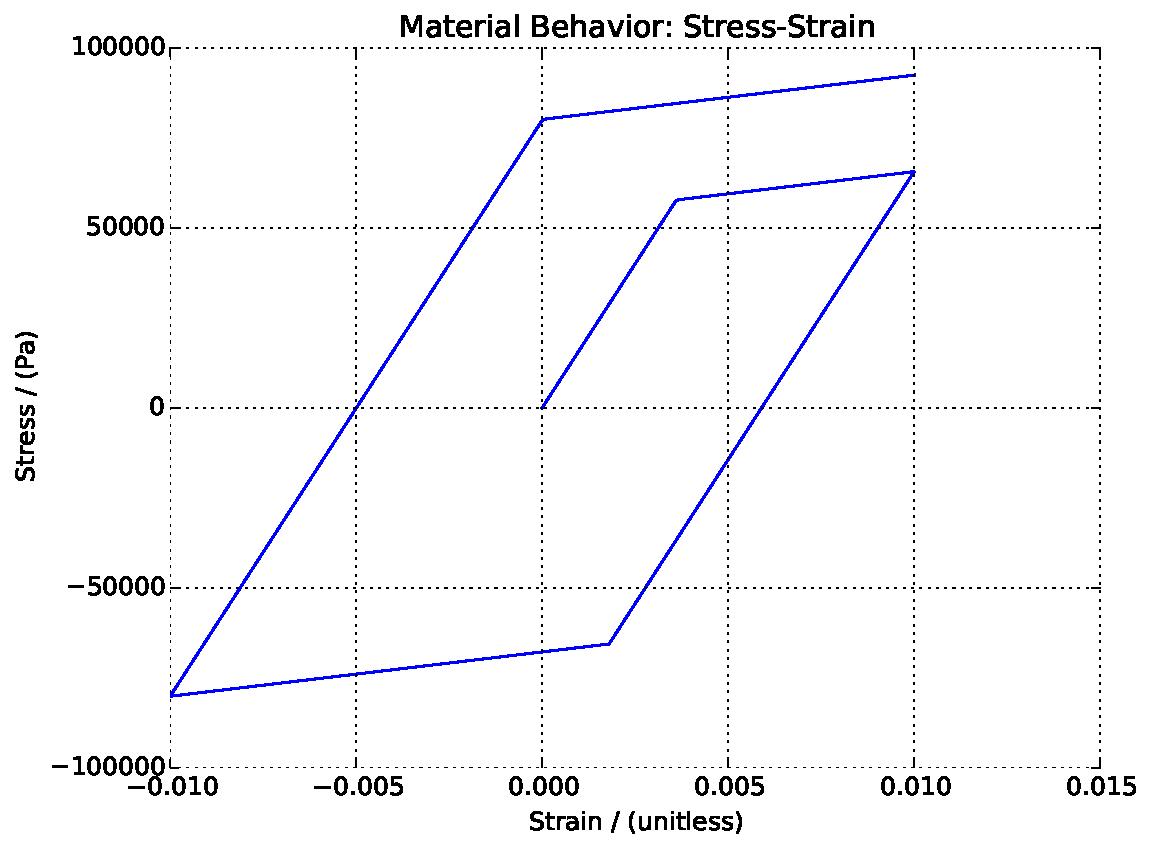
\includegraphics[width=11cm]{../fei_examples/elastoplastic_isotropic_hardening/2pure_shear_cyclic_loading/result.pdf}
\caption{
\label{Isotropic Hardening Pure Shear Cyclic Loadin}
Isotropic Hardening Pure Shear Cyclic Loading}
\end{center}
\end{figure}

The fei files for this example are available \href{https://github.com/yuan-energy/education_examples/tree/master/fei_examples/isotropic_hardening_pure_shear/2pure_shear_cyclic_loading}{here}.

%%%%%%%%%%%%%%%%%%%%%%%%%%%%%%%%%%%%%%%%%%%%%%%%%%%%%%%%%%%%%%%%%%%%%%%%%%%%
\newpage
\paragraph{Uniaxial Strain, Monotonic Loading} ~

Material Parameters:
\lstinputlisting{../fei_examples/elastoplastic_isotropic_hardening/3uniaxial_strain_mono_loading/main.fei}

Material Response:
\begin{figure}[H]
\begin{center}
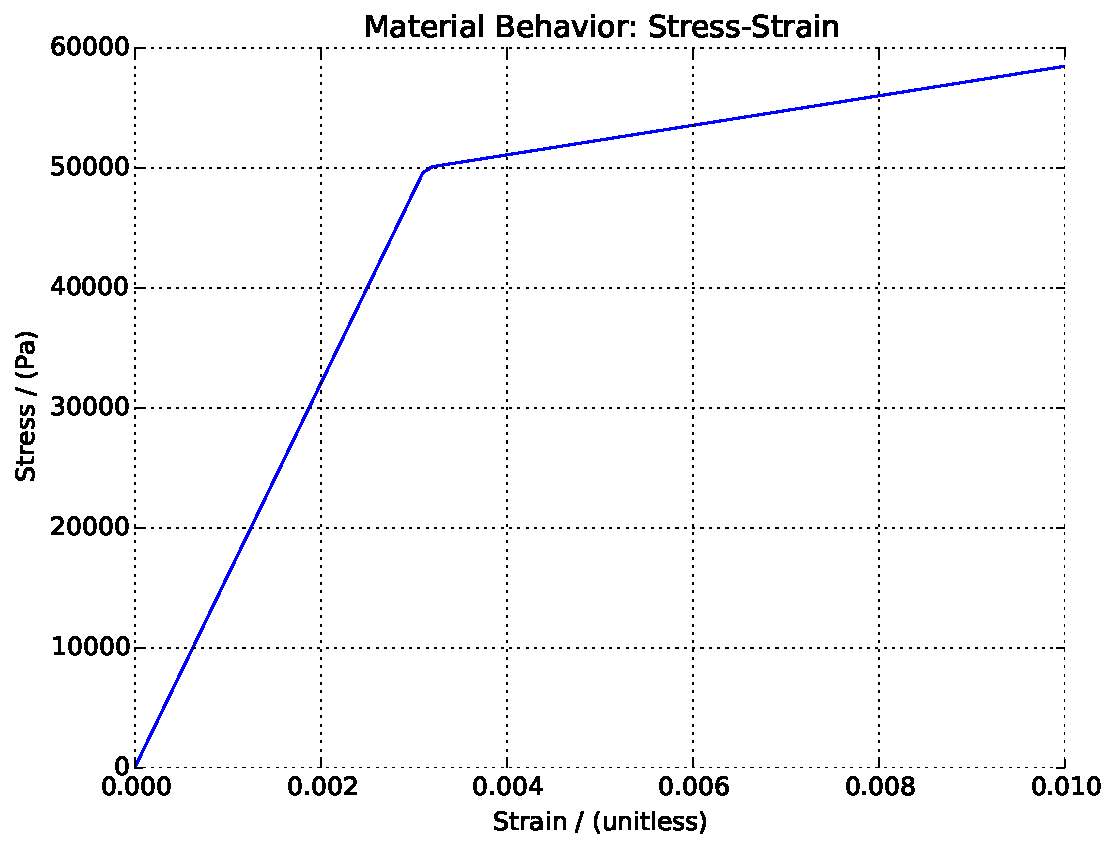
\includegraphics[width=11cm]{../fei_examples/elastoplastic_isotropic_hardening/3uniaxial_strain_mono_loading/result.pdf}
\caption{
\label{Isotropic Hardening Uniaxial Monotonic Loading}
Isotropic Hardening Uniaxial Monotonic Loading}
\end{center}
\end{figure}

The fei files for this example are available \href{https://github.com/yuan-energy/education_examples/tree/master/fei_examples/elastoplastic_isotropic_hardening/3uniaxial_strain_mono_loading}{here}.

%%%%%%%%%%%%%%%%%%%%%%%%%%%%%%%%%%%%%%%%%%%%%%%%%%%%%%%%%%%%%%%%%%%%%%%%%%%%
\newpage
\paragraph{Uniaxial Strain, Cyclic Loading} ~

Material Parameters:
\lstinputlisting{../fei_examples/elastoplastic_isotropic_hardening/4uniaxial_strain_cyclic_loading/main.fei}

Material Response:
\begin{figure}[H]
\begin{center}
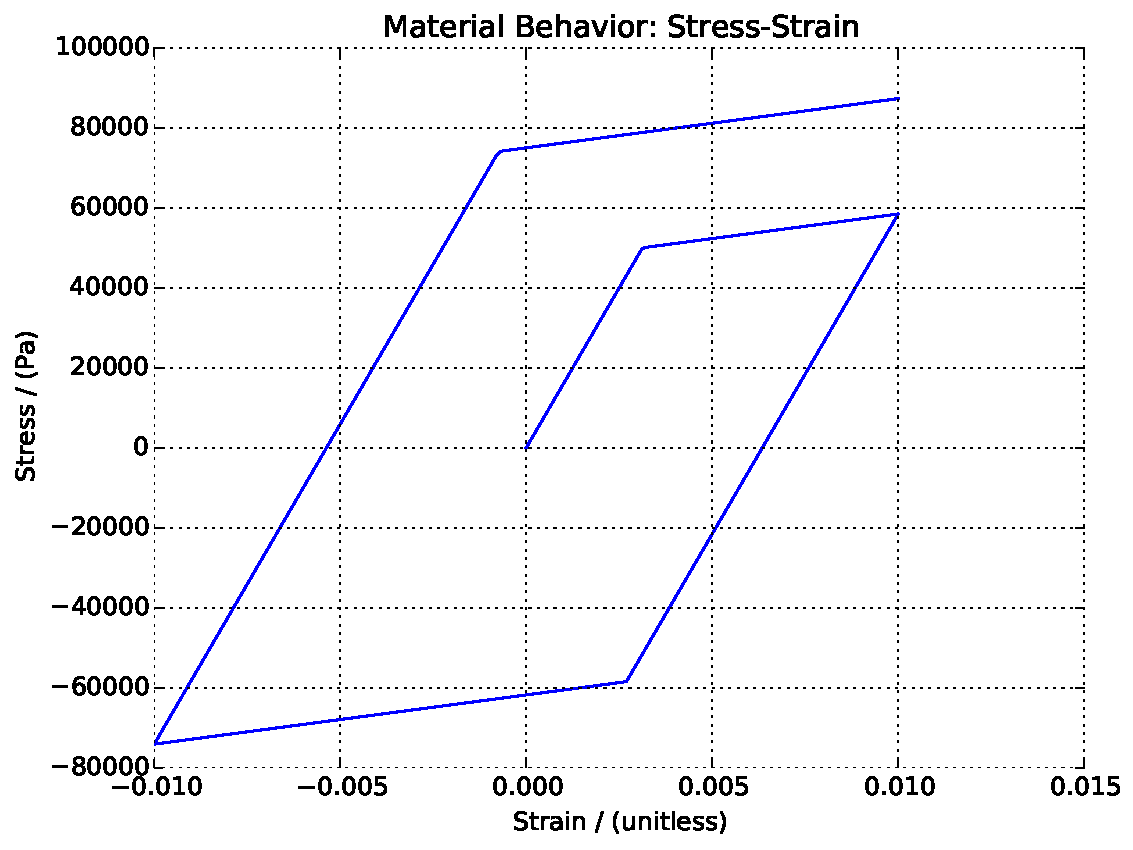
\includegraphics[width=11cm]{../fei_examples/elastoplastic_isotropic_hardening/4uniaxial_strain_cyclic_loading/result.pdf}
\caption{
\label{Isotropic Hardening Uniaxial Cyclic Loading}
Isotropic Hardening Uniaxial Cyclic Loading}
\end{center}
\end{figure}

The fei files for this example are available \href{https://github.com/yuan-energy/education_examples/tree/master/fei_examples/elastoplastic_isotropic_hardening/4uniaxial_strain_cyclic_loading}{here}.



%%%%%%%%%%%%%%%%%%%%%%%%%%%%%%%%%%%%%%%%%%%%%%%%%%%%%%%%%%%%%%%%%%%%%%%%%%%%
%%%%%%%%%%%%%%%%%%%%%%%%%%%%%%%%%%%%%%%%%%%%%%%%%%%%%%%%%%%%%%%%%%%%%%%%%%%%
%%%%%%%%%%%%%%%%%%%%%%%%%%%%%%%%%%%%%%%%%%%%%%%%%%%%%%%%%%%%%%%%%%%%%%%%%%%%
\newpage
\subsection{Elastic Plastic, Kinematic Hardening, Constitutive Examples}

%%%%%%%%%%%%%%%%%%%%%%%%%%%%%%%%%%%%%%%%%%%%%%%%%%%%%%%%%%%%%%%%%%%%%%%%%%%%
\paragraph{Pure Shear, Monotonic Loading} ~

Material Parameters:
\lstinputlisting{../fei_examples/elastoplastic_kinematic_hardening/1pure_shear_mono_loading/main.fei}

Material Response:
\begin{figure}[H]
\begin{center}
\includegraphics[width=11cm]{../fei_examples/elastoplastic_kinematic_hardening/1pure_shear_mono_loading/result.pdf}
\caption{
\label{Kinematic Hardening Monotonic Cyclic Loading}
Kinematic Hardening Monotonic Cyclic Loading}
\end{center}
\end{figure}

The fei files for this example are available \href{https://github.com/yuan-energy/education_examples/tree/master/fei_examples/kinematic_hardening_pure_shear_solid/1pure_shear_mono_loading}{here}.

%%%%%%%%%%%%%%%%%%%%%%%%%%%%%%%%%%%%%%%%%%%%%%%%%%%%%%%%%%%%%%%%%%%%%%%%%%%%
\newpage
\paragraph{Pure Shear, Cyclic Loading} ~

Material Parameters:
\lstinputlisting{../fei_examples/elastoplastic_kinematic_hardening/2pure_shear_cyclic_loading/main.fei}

Material Response:
\begin{figure}[H]
\begin{center}
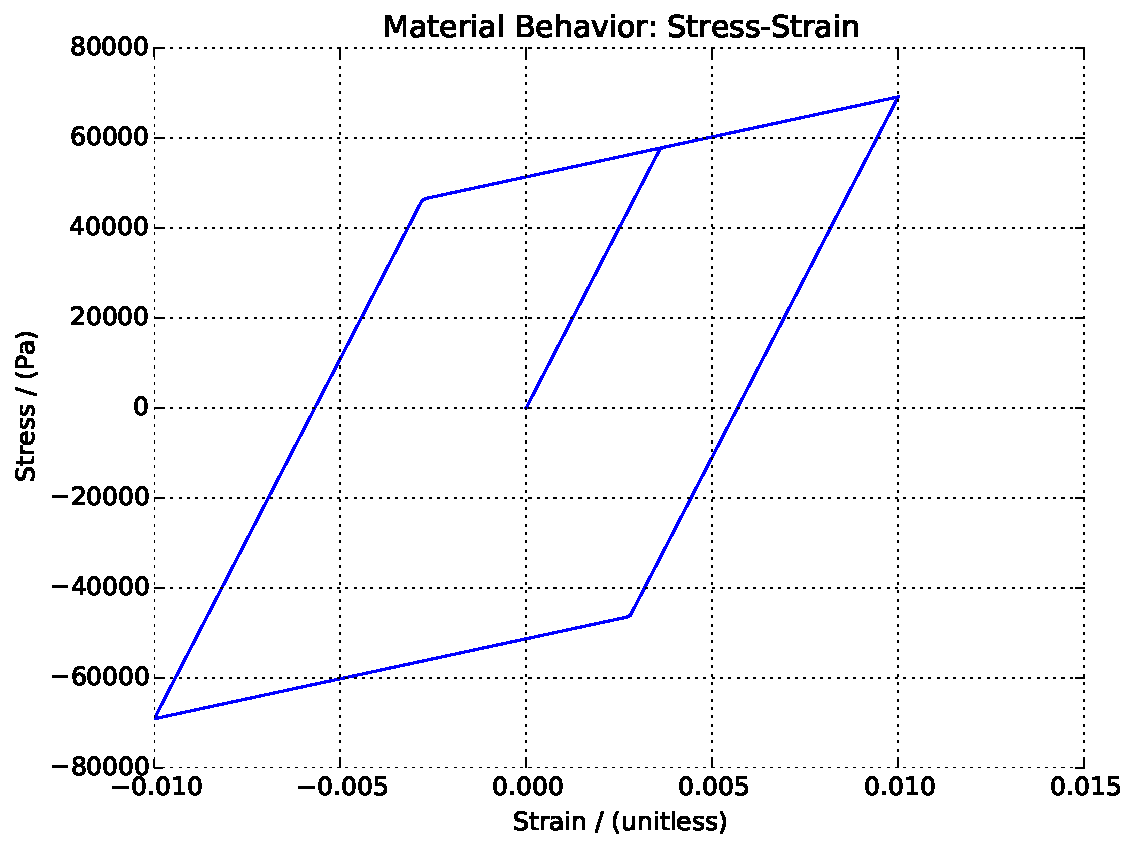
\includegraphics[width=11cm]{../fei_examples/elastoplastic_kinematic_hardening/2pure_shear_cyclic_loading/result.pdf}
\caption{
\label{Kinematic Hardening Pure Shear Cyclic Loadin}
Kinematic Hardening Pure Shear Cyclic Loading}
\end{center}
\end{figure}

The fei files for this example are available \href{https://github.com/yuan-energy/education_examples/tree/master/fei_examples/kinematic_hardening_pure_shear_solid/2pure_shear_cyclic_loading}{here}.

%%%%%%%%%%%%%%%%%%%%%%%%%%%%%%%%%%%%%%%%%%%%%%%%%%%%%%%%%%%%%%%%%%%%%%%%%%%%
\newpage
\paragraph{Uniaxial Strain, Monotonic Loading} ~

Material Parameters:
\lstinputlisting{../fei_examples/elastoplastic_kinematic_hardening/3uniaxial_strain_mono_loading/main.fei}

Material Response:
\begin{figure}[H]
\begin{center}
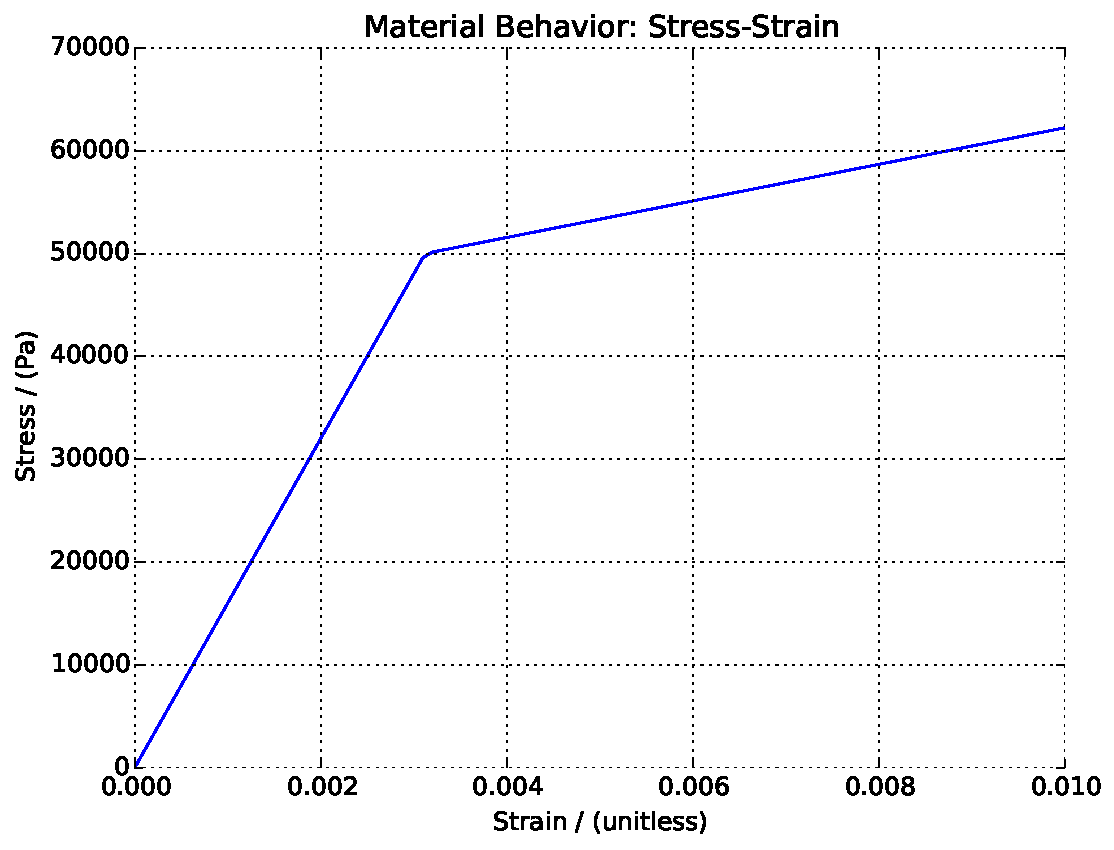
\includegraphics[width=11cm]{../fei_examples/elastoplastic_kinematic_hardening/3uniaxial_strain_mono_loading/result.pdf}
\caption{
\label{Kinematic Hardening Uniaxial Monotonic Loading}
Kinematic Hardening Uniaxial Monotonic Loading}
\end{center}
\end{figure}

The fei files for this example are available \href{https://github.com/yuan-energy/education_examples/tree/master/fei_examples/elastoplastic_kinematic_hardening/3uniaxial_strain_mono_loading}{here}.

%%%%%%%%%%%%%%%%%%%%%%%%%%%%%%%%%%%%%%%%%%%%%%%%%%%%%%%%%%%%%%%%%%%%%%%%%%%%
\newpage
\paragraph{Uniaxial Strain, Cyclic Loading} ~

Material Parameters:
\lstinputlisting{../fei_examples/elastoplastic_kinematic_hardening/4uniaxial_strain_cyclic_loading/main.fei}

Material Response:
\begin{figure}[H]
\begin{center}
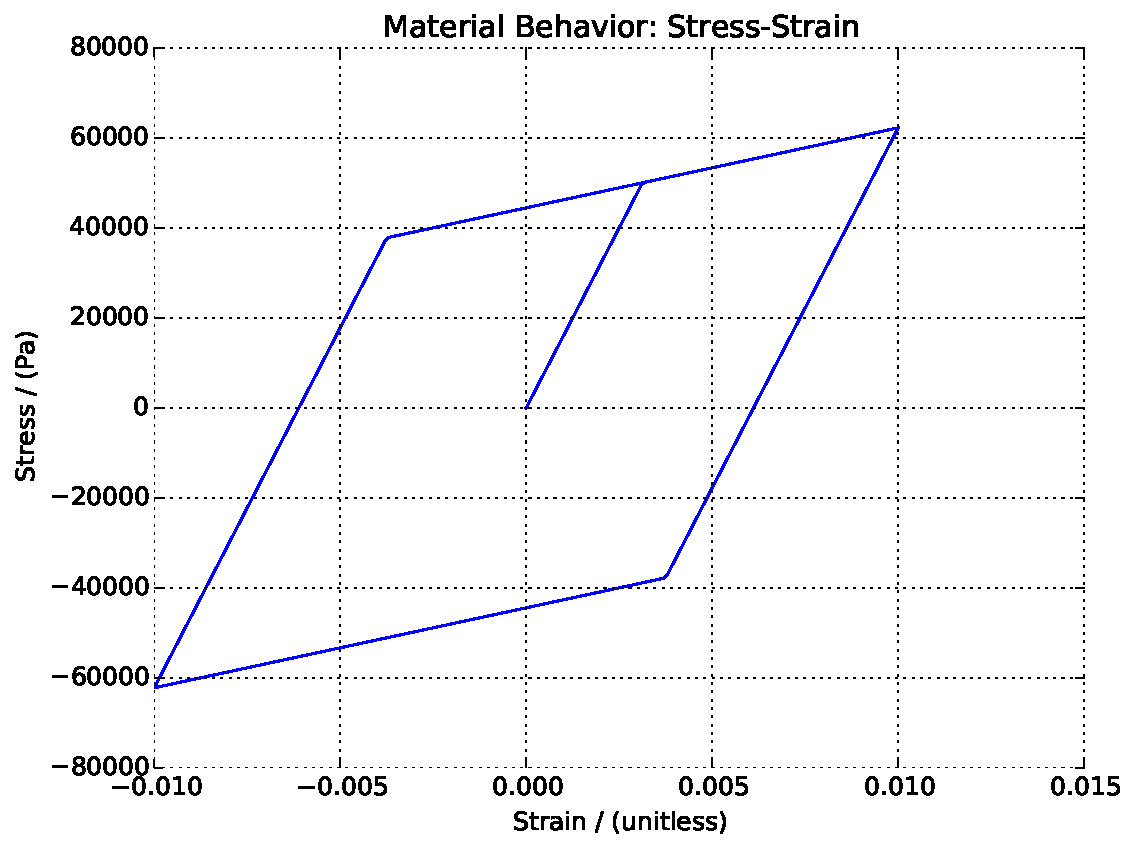
\includegraphics[width=11cm]{../fei_examples/elastoplastic_kinematic_hardening/4uniaxial_strain_cyclic_loading/result.pdf}
\caption{
\label{Kinematic Hardening Uniaxial Cyclic Loading}
Kinematic Hardening Uniaxial Cyclic Loading}
\end{center}
\end{figure}

The fei files for this example are available \href{https://github.com/yuan-energy/education_examples/tree/master/fei_examples/elastoplastic_kinematic_hardening/4uniaxial_strain_cyclic_loading}{here}.




%%%%%%%%%%%%%%%%%%%%%%%%%%%%%%%%%%%%%%%%%%%%%%%%%%%%%%%%%%%%%%%%%%%%%%%%%%%%
%%%%%%%%%%%%%%%%%%%%%%%%%%%%%%%%%%%%%%%%%%%%%%%%%%%%%%%%%%%%%%%%%%%%%%%%%%%%
%%%%%%%%%%%%%%%%%%%%%%%%%%%%%%%%%%%%%%%%%%%%%%%%%%%%%%%%%%%%%%%%%%%%%%%%%%%%
\newpage
\subsection{Elastic Plastic, Multiple Yield Surface, von-Mises, Constitutive Examples}

%%%%%%%%%%%%%%%%%%%%%%%%%%%%%%%%%%%%%%%%%%%%%%%%%%%%%%%%%%%%%%%%%%%%%%%%%%%%
\paragraph{Pure Shear, Monotonic Loading} ~

Material Parameters:
\lstinputlisting{../fei_examples/Multi_Yield_Surface_von_Mises/1pure_shear_mono_loading/main.fei}

Material Response:
\begin{figure}[H]
\begin{center}
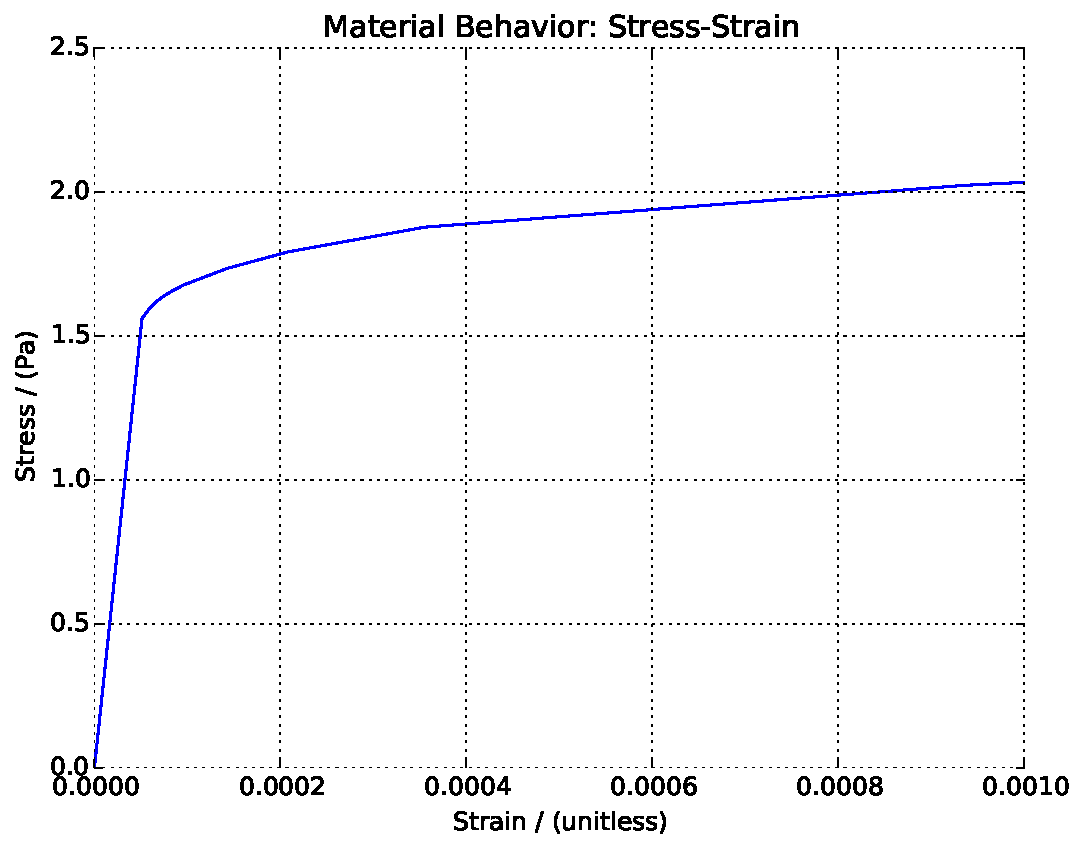
\includegraphics[width=11cm]{../fei_examples/Multi_Yield_Surface_von_Mises/1pure_shear_mono_loading/result.pdf}
\caption{
\label{Multiple Yield Surface Pure Shear Monotoni}
Multiple Yield Surface Pure Shear Monotonic Loading}
\end{center}
\end{figure}

The fei files for this example are available \href{https://github.com/yuan-energy/education_examples/tree/master/fei_examples/Multi_Yield_Surface_von_Mises/1pure_shear_mono_loading}{here}.

%%%%%%%%%%%%%%%%%%%%%%%%%%%%%%%%%%%%%%%%%%%%%%%%%%%%%%%%%%%%%%%%%%%%%%%%%%%%
\newpage
\paragraph{Pure Shear, Cyclic Loading} ~

Material Parameters:
\lstinputlisting{../fei_examples/Multi_Yield_Surface_von_Mises/2pure_shear_cyclic_loading/main.fei}

Material Response:
\begin{figure}[H]
\begin{center}
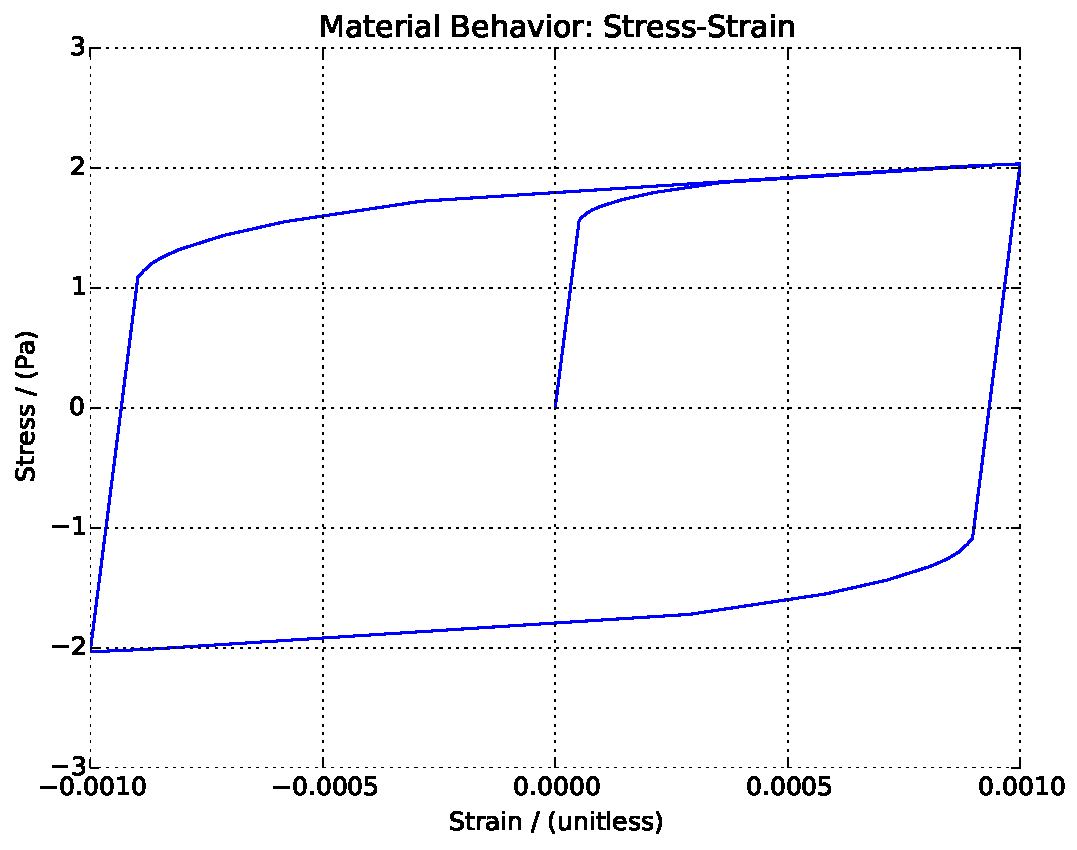
\includegraphics[width=11cm]{../fei_examples/Multi_Yield_Surface_von_Mises/2pure_shear_cyclic_loading/result.pdf}
\caption{
\label{Multiple Yield Surface Pure Shear Cycli}
Multiple Yield Surface Pure Shear Cyclic Loading}
\end{center}
\end{figure}

The fei files for this example are available \href{https://github.com/yuan-energy/education_examples/tree/master/fei_examples/Multi_Yield_Surface_von_Mises/2pure_shear_cyclic_loading}{here}.

















%%%%%%%%%%%%%%%%%%%%%%%%%%%%%%%%%%%%%%%%%%%%%%%%%%%%%%%%%%%%%%%%%%%%%%%%%%%%
%%%%%%%%%%%%%%%%%%%%%%%%%%%%%%%%%%%%%%%%%%%%%%%%%%%%%%%%%%%%%%%%%%%%%%%%%%%%
%%%%%%%%%%%%%%%%%%%%%%%%%%%%%%%%%%%%%%%%%%%%%%%%%%%%%%%%%%%%%%%%%%%%%%%%%%%%
%%%%%%%%%%%%%%%%%%%%%%%%%%%%%%%%%%%%%%%%%%%%%%%%%%%%%%%%%%%%%%%%%%%%%%%%%%%%
%%%%%%%%%%%%%%%%%%%%%%%%%%%%%%%%%%%%%%%%%%%%%%%%%%%%%%%%%%%%%%%%%%%%%%%%%%%%
%%%%%%%%%%%%%%%%%%%%%%%%%%%%%%%%%%%%%%%%%%%%%%%%%%%%%%%%%%%%%%%%%%%%%%%%%%%%
%%%%%%%%%%%%%%%%%%%%%%%%%%%%%%%%%%%%%%%%%%%%%%%%%%%%%%%%%%%%%%%%%%%%%%%%%%%%
\newpage
\section{Elastic Single Solid Finite Finite Element Examples}
\label{section_elastic_brick_example}
%%%%%%%%%%%%%%%%%%%%%%%%%%%%%%%%%%%%%%%%%%%%%%%%%%%%%%%%%%%%%%%%%%%%%%%%%%%%
\subsection{Linear Elastic, Solid Examples}

%%%%%%%%%%%%%%%%%%%%%%%%%%%%%%%%%%%%%%%%%%%%%%%%%%%%%%%%%%%%%%%%%%%%%%%%%%%%
\paragraph{Pure Shear, Monotonic Loading} ~

Model Description:

\begin{figure}[H]
\begin{center}
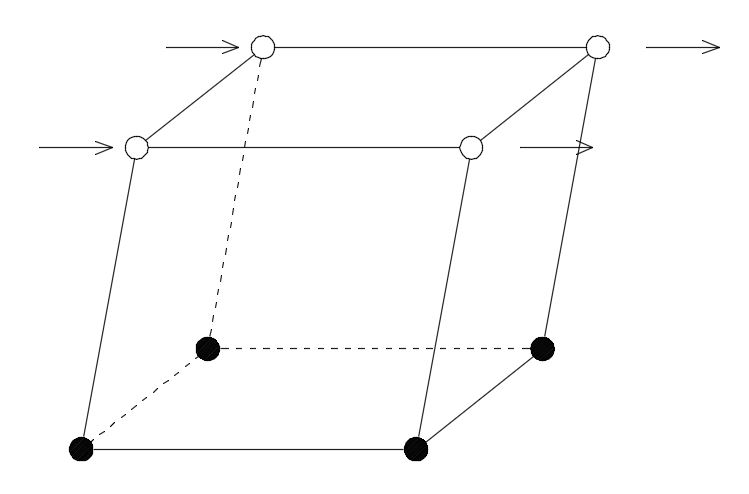
\includegraphics[width=8cm]{../Figure-files/shear_brick.JPG}
\caption{
\label{Diagram_Linear Elastic Pure Shear Monotonic Loadin}
Diagram Linear Elastic Solid Pure Shear Monotonic Loading}
\end{center}
\end{figure}

Material Response at Gauss Point:
\begin{figure}[H]
\begin{center}
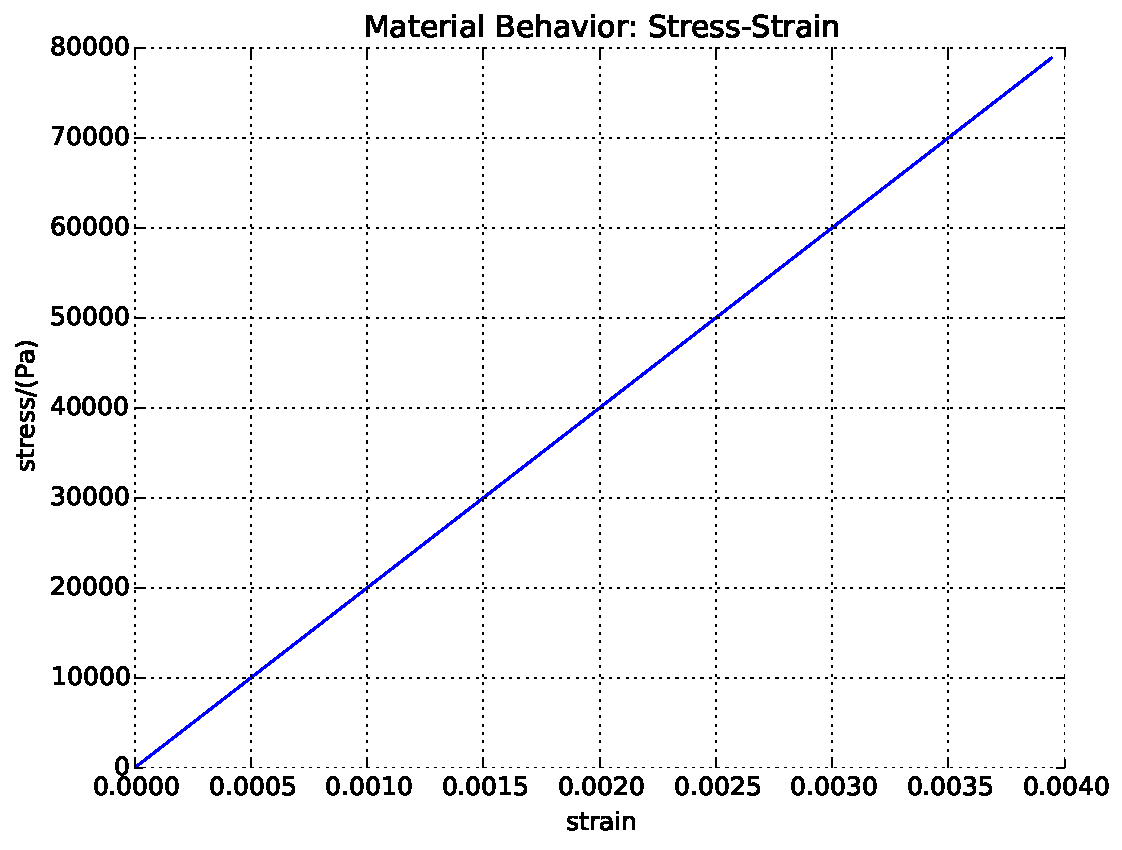
\includegraphics[width=11cm]{../fei_examples/linear_elastic_solid/1pure_shear_mono_loading/result.pdf}
\caption{
\label{Linear Elastic_solid Pure Shear Monotonic Loadin}
Results of Linear Elastic Solid Pure Shear Monotonic Loading}
\end{center}
\end{figure}

The fei files for this example are available \href{https://github.com/yuan-energy/education_examples/tree/master/fei_examples/linear_elastic_solid/1pure_shear_mono_loading}{here}.

%%%%%%%%%%%%%%%%%%%%%%%%%%%%%%%%%%%%%%%%%%%%%%%%%%%%%%%%%%%%%%%%%%%%%%%%%%%%
\newpage
\paragraph{Pure Shear, Cyclic Loading} ~

Model Description:

\begin{figure}[H]
\begin{center}
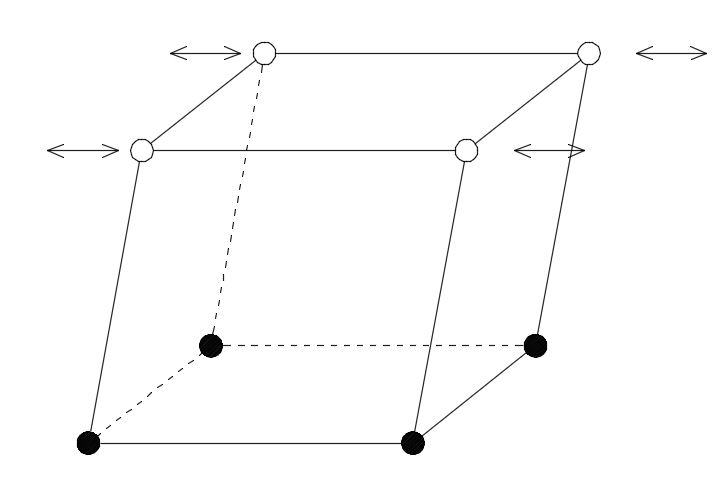
\includegraphics[width=8cm]{../Figure-files/shear_cyclic_brick.JPG}
\caption{
\label{Solid Linear Elastic Solid Pure Shear Cyclic Loadin}
Diagram Linear Elastic Solid Pure Shear Cyclic Loading}
\end{center}
\end{figure}

Material Response at Gauss Point:
\begin{figure}[H]
\begin{center}
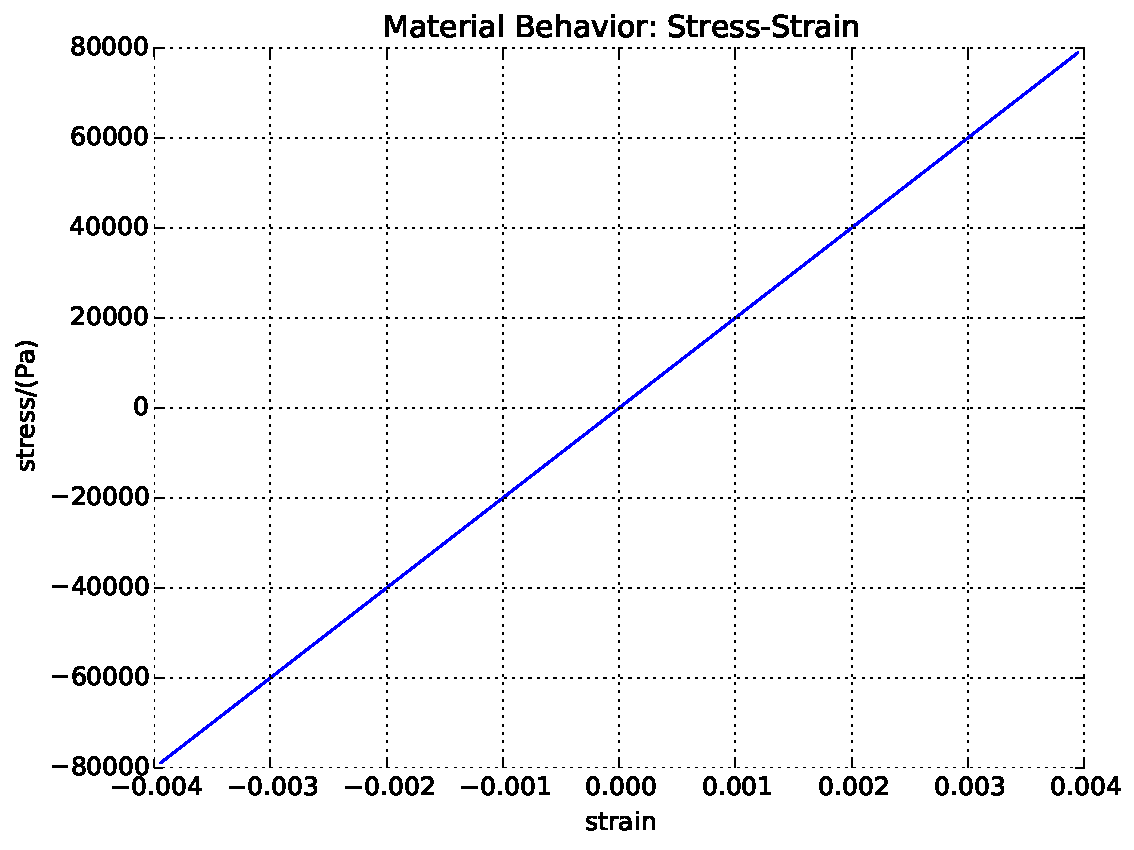
\includegraphics[width=11cm]{../fei_examples/linear_elastic_solid/2pure_shear_cyclic_loading/result.pdf}
\caption{
\label{Results Linear Elastic Solid Pure Shear Cyclic Loadin}
Results of Linear Elastic Solid Pure Shear Cyclic Loading}
\end{center}
\end{figure}

The fei files for this example are available \href{https://github.com/yuan-energy/education_examples/tree/master/fei_examples/linear_elastic_solid/2pure_shear_cyclic_loading}{here}.


% %%%%%%%%%%%%%%%%%%%%%%%%%%%%%%%%%%%%%%%%%%%%%%%%%%%%%%%%%%%%%%%%%%%%%%%%%%%%
\newpage
\paragraph{Uniaxial Strain, Monotonic Loading} ~

Model Description:

\begin{figure}[H]
\begin{center}
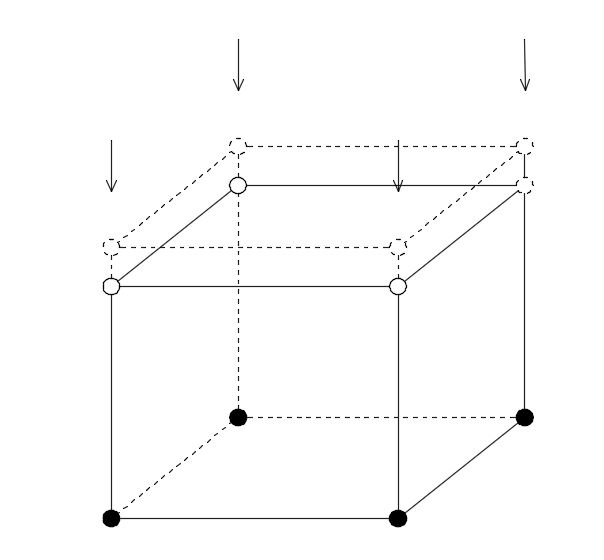
\includegraphics[width=8cm]{../Figure-files/vertical.JPG}
\caption{
\label{Diagram Linear Elastic Uniaxial Strain Solid Monotonic Loadin}
Diagram Linear Elastic Uniaxial Strain Solid Monotonic Loading}
\end{center}
\end{figure}

Material Response at Gauss Point:
\begin{figure}[H]
\begin{center}
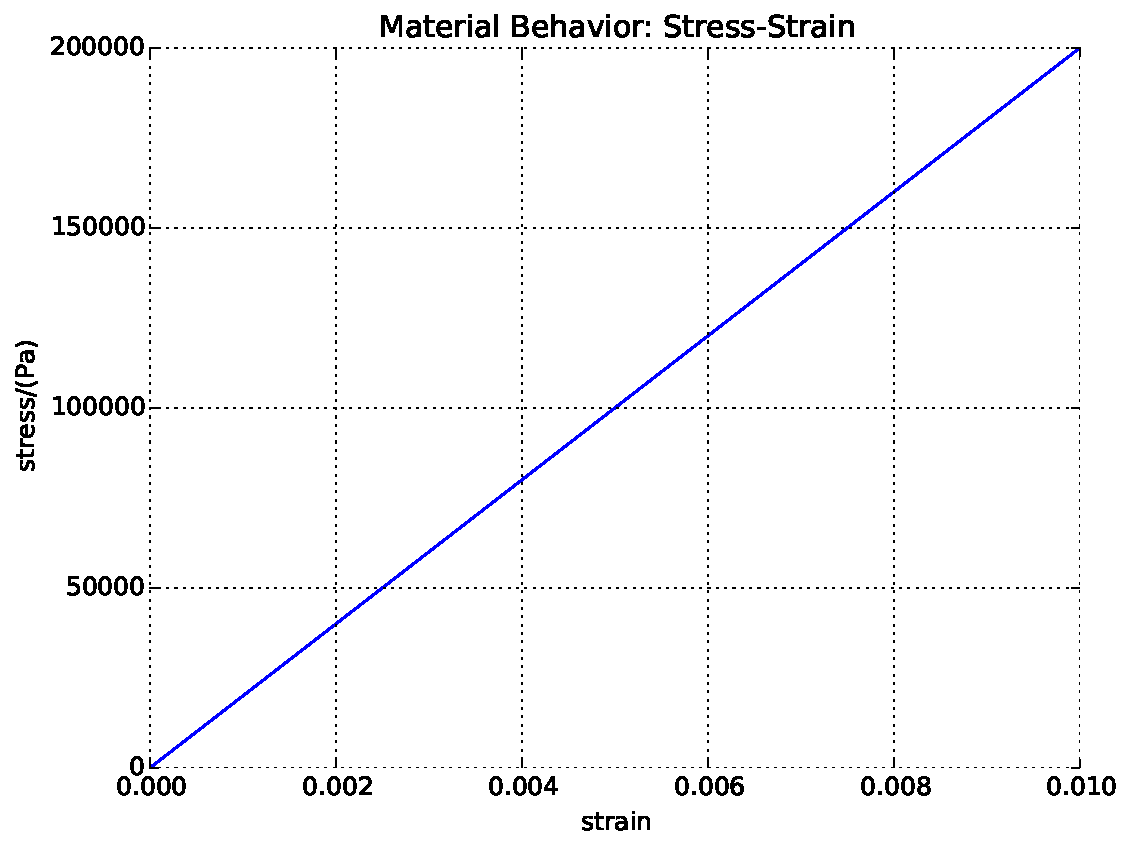
\includegraphics[width=11cm]{../fei_examples/linear_elastic_solid/3uniaxial_strain_mono_loading/result.pdf}
\caption{
\label{Results of Linear Elastic Solid Pure Shear Cyclic Loadin}
Results of Linear Elastic Pure Shear Cyclic Loading}
\end{center}
\end{figure}

The fei files for this example are available \href{https://github.com/yuan-energy/education_examples/tree/master/fei_examples/linear_elastic_solid/3uniaxial_strain_mono_loading}{here}.


% %%%%%%%%%%%%%%%%%%%%%%%%%%%%%%%%%%%%%%%%%%%%%%%%%%%%%%%%%%%%%%%%%%%%%%%%%%%%
\newpage
\paragraph{Uniaxial Strain, Cyclic Loading} ~

Model Description:

\begin{figure}[H]
\begin{center}
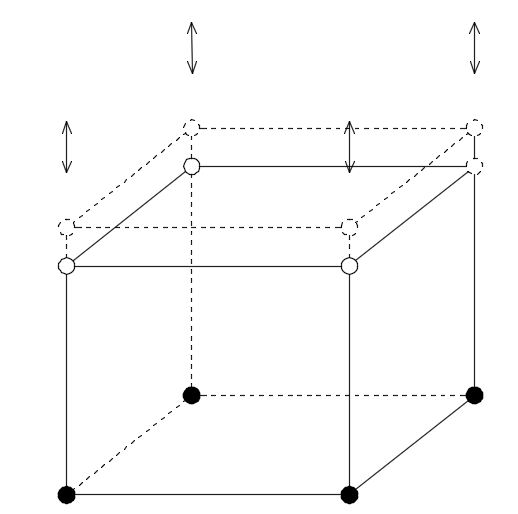
\includegraphics[width=8cm]{../Figure-files/vertical_cyclic.JPG}
\caption{
\label{Linear Elastic Uniaxial Strain Cyclic Loadin}
Linear Elastic Uniaxial Strain Cyclic Loading}
\end{center}
\end{figure}

Material Response at Gauss Point:

\begin{figure}[H]
\begin{center}
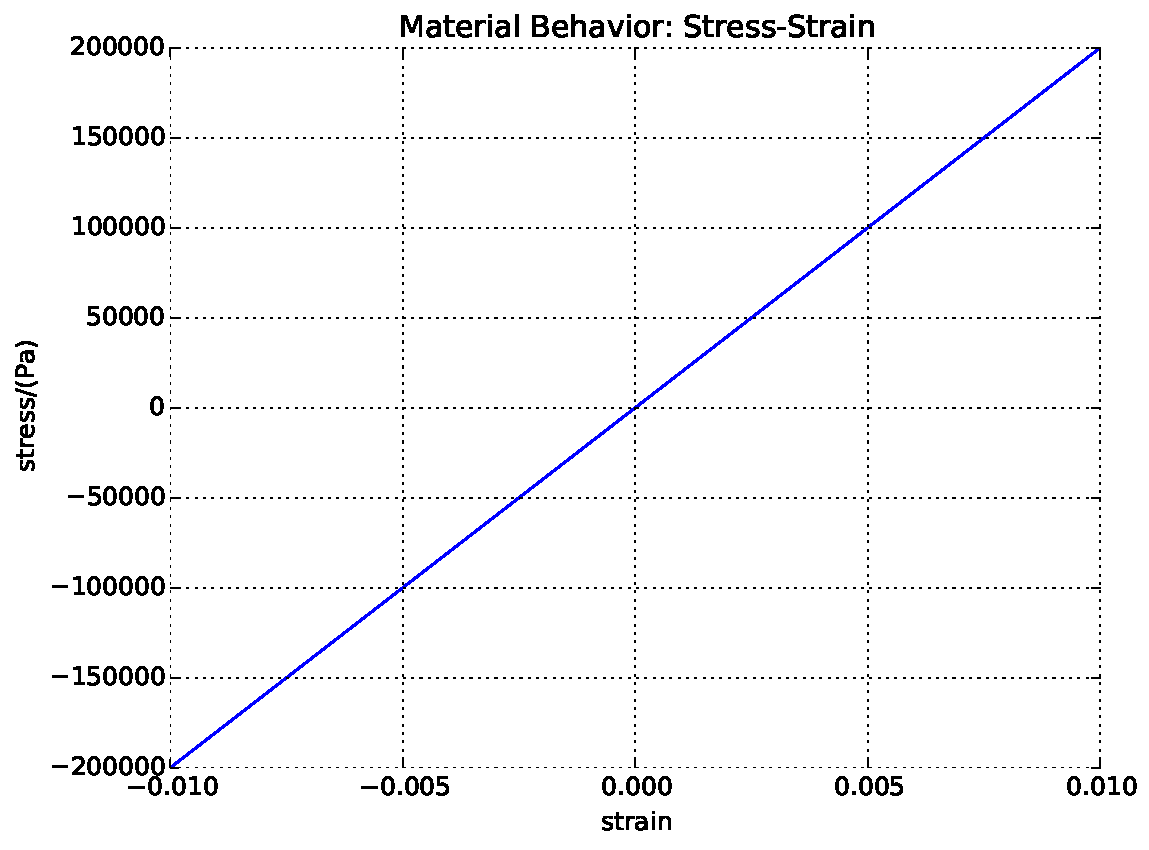
\includegraphics[width=11cm]{../fei_examples/linear_elastic_solid/4uniaxial_strain_cyclic_loading/result.pdf}
\caption{
\label{Results_Linear Elastic Pure Shear Cyclic Loadin}
Results of Linear Elastic Pure Shear Cyclic Loading}
\end{center}
\end{figure}

The fei files for this example are available \href{https://github.com/yuan-energy/education_examples/tree/master/fei_examples/linear_elastic_solid/4uniaxial_strain_cyclic_loading}{here}.


%%%%%%%%%%%%%%%%%%%%%%%%%%%%%%%%%%%%%%%%%%%%%%%%%%%%%%%%%%%%%%%%%%%%%%%%%%%%
%%%%%%%%%%%%%%%%%%%%%%%%%%%%%%%%%%%%%%%%%%%%%%%%%%%%%%%%%%%%%%%%%%%%%%%%%%%%
%%%%%%%%%%%%%%%%%%%%%%%%%%%%%%%%%%%%%%%%%%%%%%%%%%%%%%%%%%%%%%%%%%%%%%%%%%%%
% \newpage
% \subsection{Nonlinear Elastic Pure Shear Solid Examples}

% %%%%%%%%%%%%%%%%%%%%%%%%%%%%%%%%%%%%%%%%%%%%%%%%%%%%%%%%%%%%%%%%%%%%%%%%%%%%
% \paragraph{Pure Shear, Monotonic Loading} ~

% %%%%%%%%%%%%%%%%%%%%%%%%%%%%%%%%%%%%%%%%%%%%%%%%%%%%%%%%%%%%%%%%%%%%%%%%%%%%
% \paragraph{Pure Shear, Cyclic Loading} ~


% %%%%%%%%%%%%%%%%%%%%%%%%%%%%%%%%%%%%%%%%%%%%%%%%%%%%%%%%%%%%%%%%%%%%%%%%%%%%
% \paragraph{Uniaxial Strain, Monotonic Loading} ~

% %%%%%%%%%%%%%%%%%%%%%%%%%%%%%%%%%%%%%%%%%%%%%%%%%%%%%%%%%%%%%%%%%%%%%%%%%%%%
% \paragraph{Uniaxial Strain, Cyclic Loading} ~











% %%%%%%%%%%%%%%%%%%%%%%%%%%%%%%%%%%%%%%%%%%%%%%%%%%%%%%%%%%%%%%%%%%%%%%%%%%%%
% %%%%%%%%%%%%%%%%%%%%%%%%%%%%%%%%%%%%%%%%%%%%%%%%%%%%%%%%%%%%%%%%%%%%%%%%%%%%
% %%%%%%%%%%%%%%%%%%%%%%%%%%%%%%%%%%%%%%%%%%%%%%%%%%%%%%%%%%%%%%%%%%%%%%%%%%%%
% %%%%%%%%%%%%%%%%%%%%%%%%%%%%%%%%%%%%%%%%%%%%%%%%%%%%%%%%%%%%%%%%%%%%%%%%%%%%
% %%%%%%%%%%%%%%%%%%%%%%%%%%%%%%%%%%%%%%%%%%%%%%%%%%%%%%%%%%%%%%%%%%%%%%%%%%%%
% %%%%%%%%%%%%%%%%%%%%%%%%%%%%%%%%%%%%%%%%%%%%%%%%%%%%%%%%%%%%%%%%%%%%%%%%%%%%
\newpage
\section{Elastic-Plastic Single Solid Finite Element Examples}
\label{section_elastoplastic_brick_example}
% %%%%%%%%%%%%%%%%%%%%%%%%%%%%%%%%%%%%%%%%%%%%%%%%%%%%%%%%%%%%%%%%%%%%%%%%%%%%
% %%%%%%%%%%%%%%%%%%%%%%%%%%%%%%%%%%%%%%%%%%%%%%%%%%%%%%%%%%%%%%%%%%%%%%%%%%%%
\subsection{Elastic Perfectly Plastic, Cyclic Loading, Pure Shear Solid Examples}

Model Description:

\begin{figure}[H]
\begin{center}
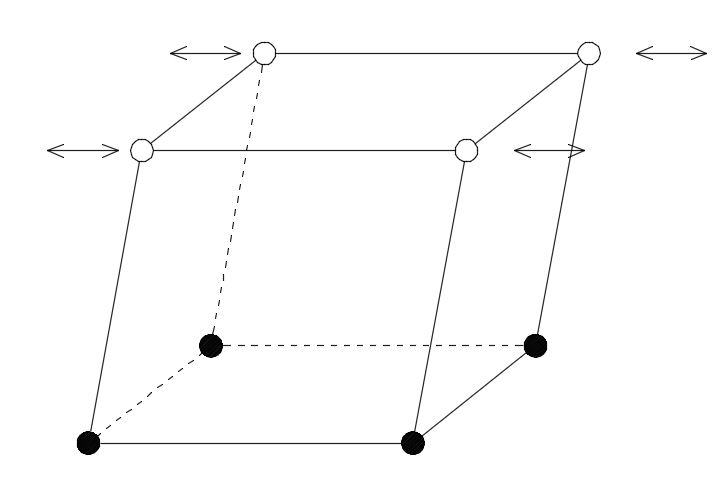
\includegraphics[width=8cm]{../Figure-files/shear_cyclic_brick.JPG}
\caption{
\label{Perfectly Plastic Pure Shear Cyclic Loadin}
Perfectly Plastic Pure Shear Cyclic Loading}
\end{center}
\end{figure}

Material Response at Gauss Point:

\begin{figure}[H]
\begin{center}
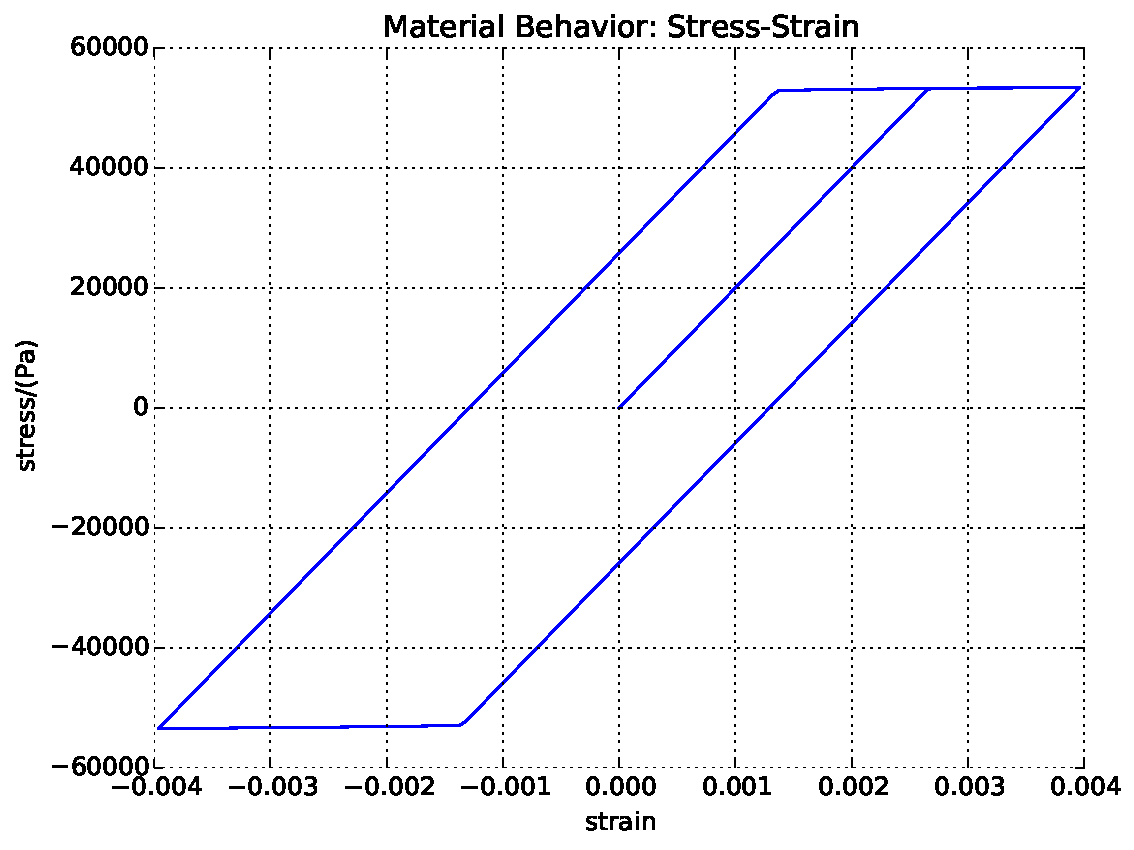
\includegraphics[width=11cm]{../fei_examples/perfectly_plastic_pure_shear_solid/2pure_shear_cyclic_loading/result.pdf}
\caption{
\label{Results of Linear Elastic Pure Shear Cyclic Loadin}
Results of Linear Elastic Pure Shear Cyclic Loading}
\end{center}
\end{figure}

The fei files for this example are available \href{https://github.com/yuan-energy/education_examples/tree/master/fei_examples/perfectly_plastic_pure_shear_solid/2pure_shear_cyclic_loading}{here}.


% %%%%%%%%%%%%%%%%%%%%%%%%%%%%%%%%%%%%%%%%%%%%%%%%%%%%%%%%%%%%%%%%%%%%%%%%%%%%
\newpage
\subsubsection{von Mises Yield Function, Isotropic Hardening} ~

Model Description:

\begin{figure}[H]
\begin{center}
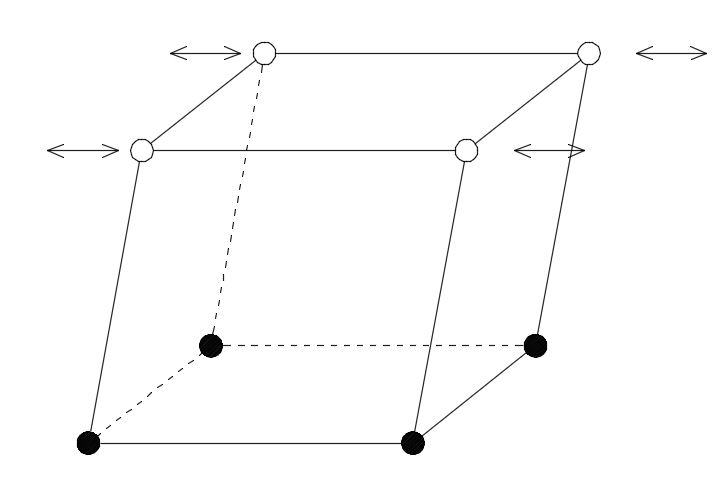
\includegraphics[width=8cm]{../Figure-files/shear_cyclic_brick.JPG}
\caption{
\label{vmih Linear Elastic Pure Shear Cyclic Loadin}
Linear Elastic Pure Shear Cyclic Loading}
\end{center}
\end{figure}

Material Response at Gauss Point:

\begin{figure}[H]
\begin{center}
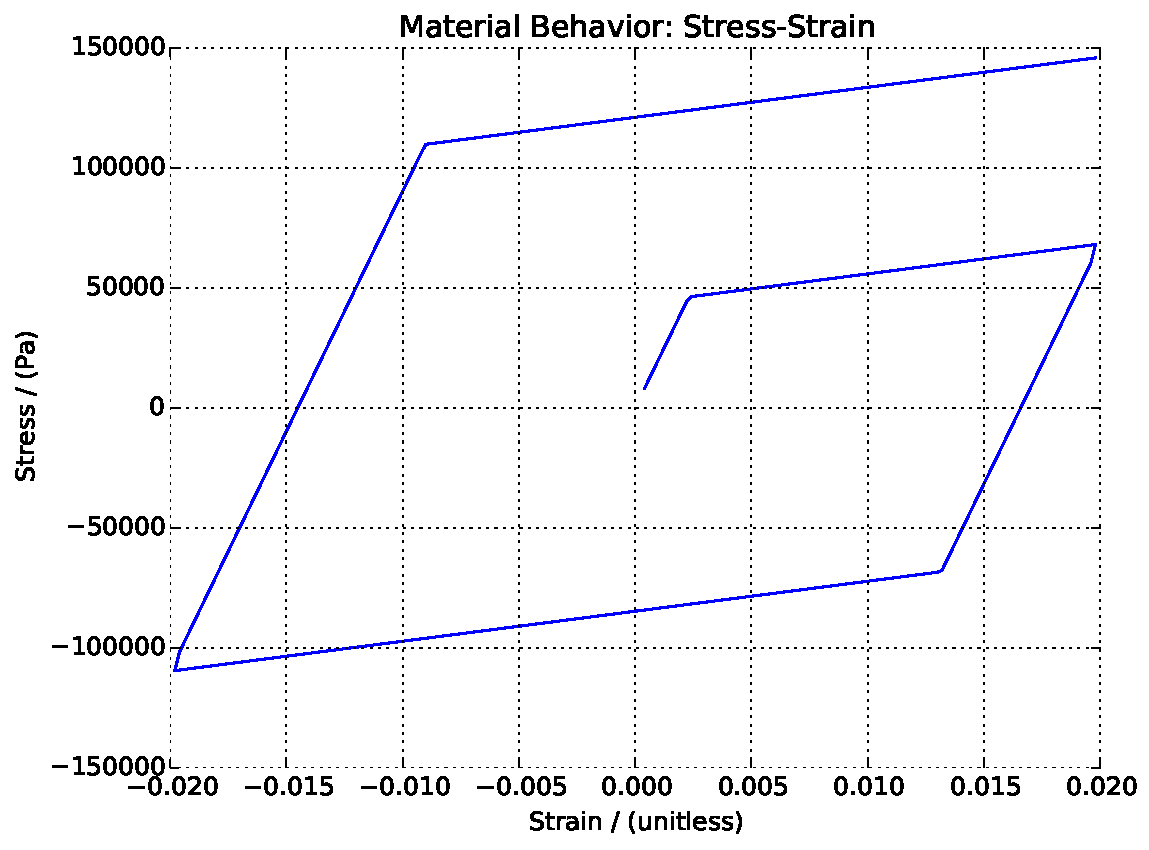
\includegraphics[width=11cm]{../fei_examples/isotropic_hardening_pure_shear/2pure_shear_cyclic_loading/result.pdf}
\caption{
\label{Results_vmih_Linear Elastic Pure Shear Cyclic Loadin}
Linear Elastic Pure Shear Cyclic Loading}
\end{center}
\end{figure}

The fei files for this example are available \href{https://github.com/yuan-energy/education_examples/tree/master/fei_examples/isotropic_hardening_pure_shear/2pure_shear_cyclic_loading}{here}.


% % %%%%%%%%%%%%%%%%%%%%%%%%%%%%%%%%%%%%%%%%%%%%%%%%%%%%%%%%%%%%%%%%%%%%%%%%%%%%
\newpage
\subsubsection{von Mises Yield Function, Kinematic Hardening} ~

Model Description:

\begin{figure}[H]
\begin{center}
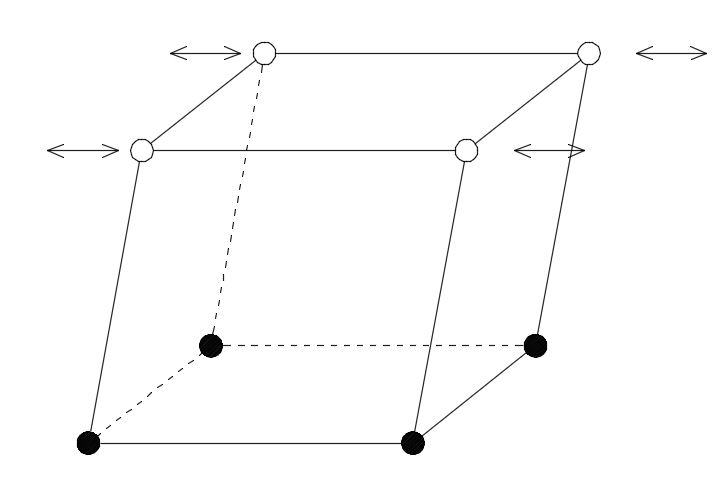
\includegraphics[width=8cm]{../Figure-files/shear_cyclic_brick.JPG}
\caption{
\label{von Mises Pure Shear Cyclic Loadin}
von Mises Pure Shear Cyclic Loading}
\end{center}
\end{figure}

Material Response at Gauss Point:

\begin{figure}[H]
\begin{center}
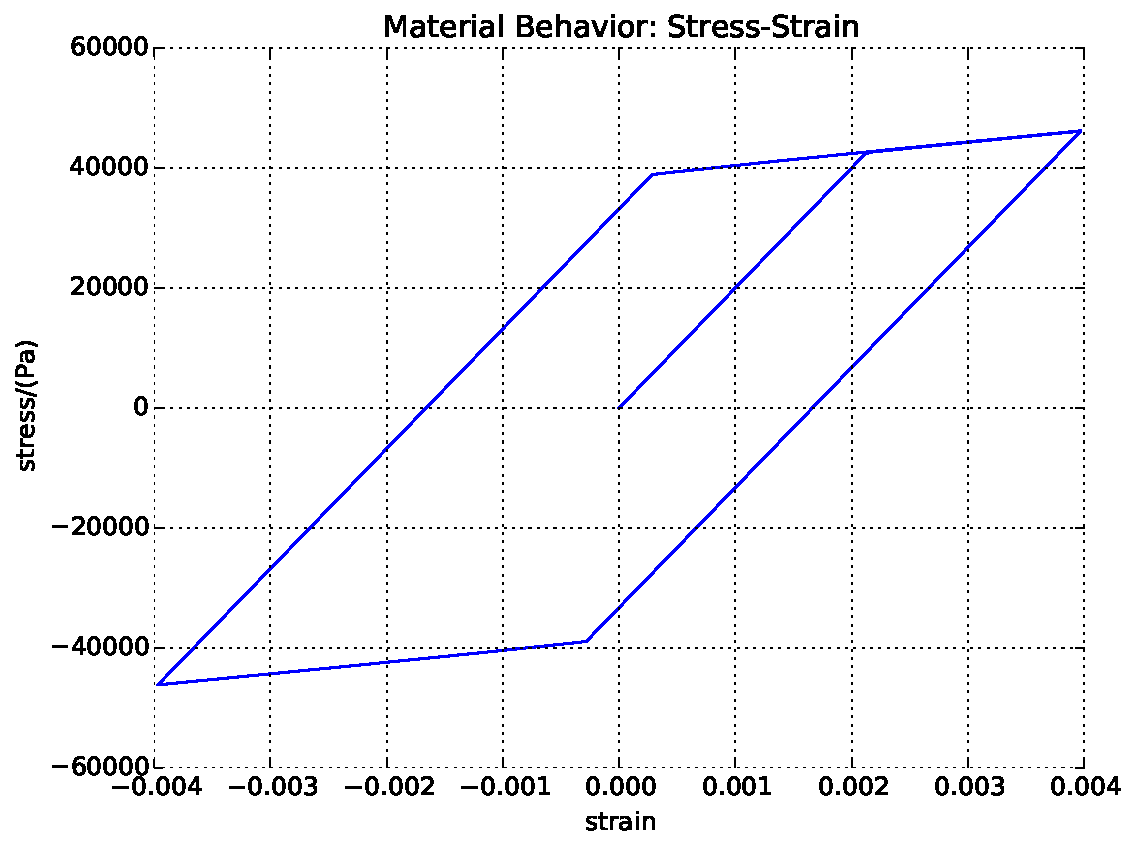
\includegraphics[width=11cm]{../fei_examples/kinematic_hardening_pure_shear_solid/2pure_shear_cyclic_loading/result.pdf}
\caption{
\label{Results of von Mises Pure Shear Cyclic Loadin}
Results of von Mises Pure Shear Cyclic Loading}
\end{center}
\end{figure}

The fei files for this example are available \href{https://github.com/yuan-energy/education_examples/tree/master/fei_examples/kinematic_hardening_pure_shear_solid/2pure_shear_cyclic_loading}{here}.

% % %%%%%%%%%%%%%%%%%%%%%%%%%%%%%%%%%%%%%%%%%%%%%%%%%%%%%%%%%%%%%%%%%%%%%%%%%%%%
\newpage
\subsubsection{Drucker Prager Yield Function, von Mises Plastic Potential Function, Perfectly Plastic Hardening Rule} ~

Model Description:

\begin{figure}[H]
\begin{center}
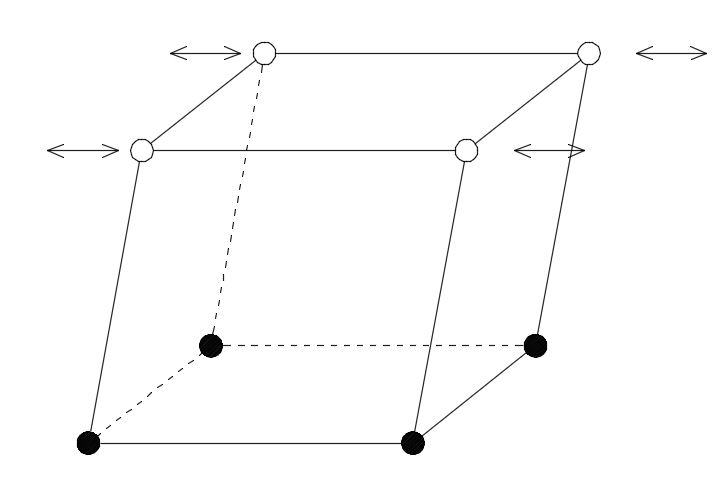
\includegraphics[width=8cm]{../Figure-files/shear_cyclic_brick.JPG}
\caption{
\label{Diagram Non-associative Drucker Prager Pure Shear Cyclic Loadin}
Diagram of Non-associative Drucker Prager Pure Shear Cyclic Loading}
\end{center}
\end{figure}


\begin{figure}[H]
\begin{center}
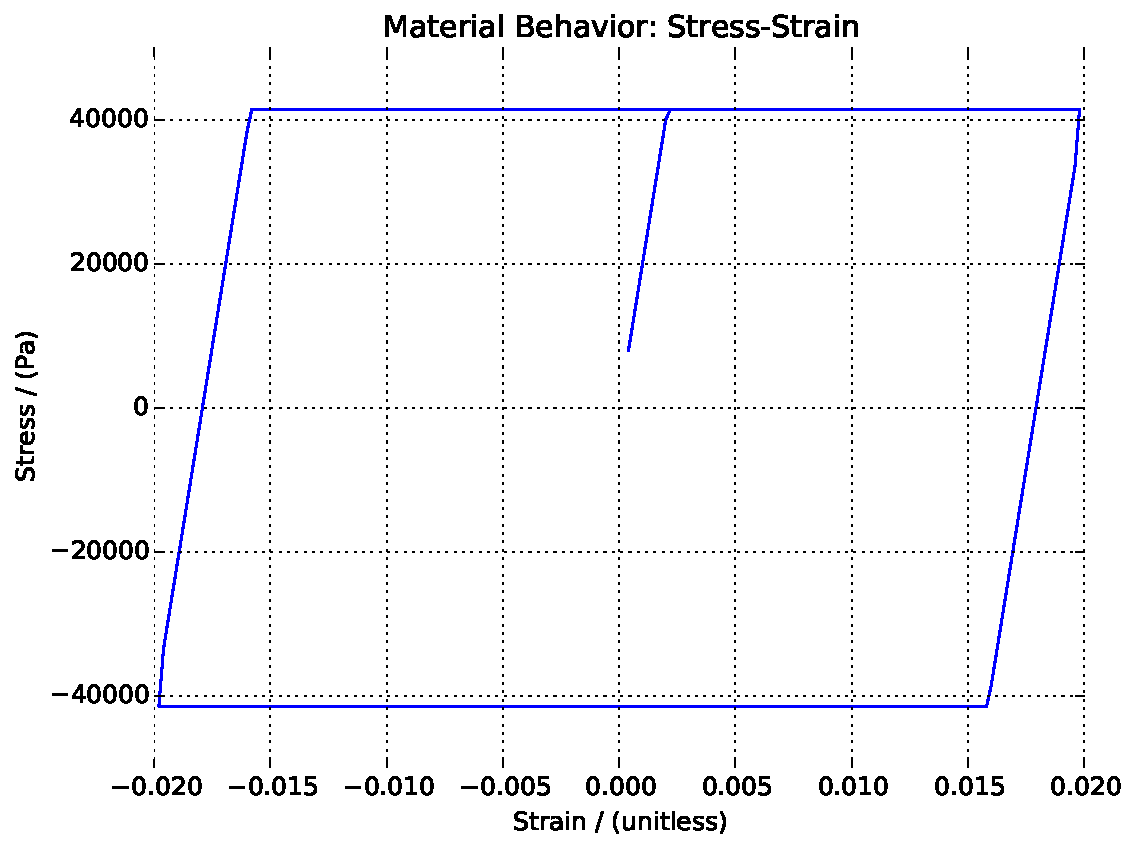
\includegraphics[width=11cm]{../fei_examples/Drucker_Prager_Non_associate_Flow_Solid/2pure_shear_cyclic_loading/result.pdf}
\caption{
\label{Results of Drucker Prager Pure Shear Cyclic Loadin}
Results of Drucker Prager Pure Shear Cyclic Loading}
\end{center}
\end{figure}

The fei files for this example are available \href{https://github.com/yuan-energy/education_examples/tree/master/fei_examples/Drucker_Prager_Non_associate_Flow_Solid/2pure_shear_cyclic_loading}{here}.


% % %%%%%%%%%%%%%%%%%%%%%%%%%%%%%%%%%%%%%%%%%%%%%%%%%%%%%%%%%%%%%%%%%%%%%%%%%%%%
\newpage
\subsubsection{Drucker Prager Yield Function, Drucker Prager Plastic Potential Function, Perfectly Plastic Hardening Rule} ~ 

Model Description:

\begin{figure}[H]
\begin{center}
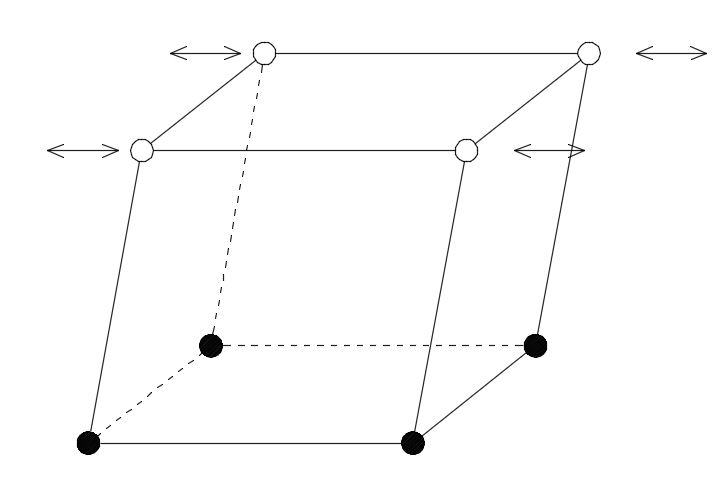
\includegraphics[width=8cm]{../Figure-files/shear_cyclic_brick.JPG}
\caption{
\label{Associative Drucker Prager Pure Shear Cyclic Loadin}
Associative Drucker Prager Pure Shear Cyclic Loading}
\end{center}
\end{figure}

Material Response at Gauss Point:

\begin{figure}[H]
\begin{center}
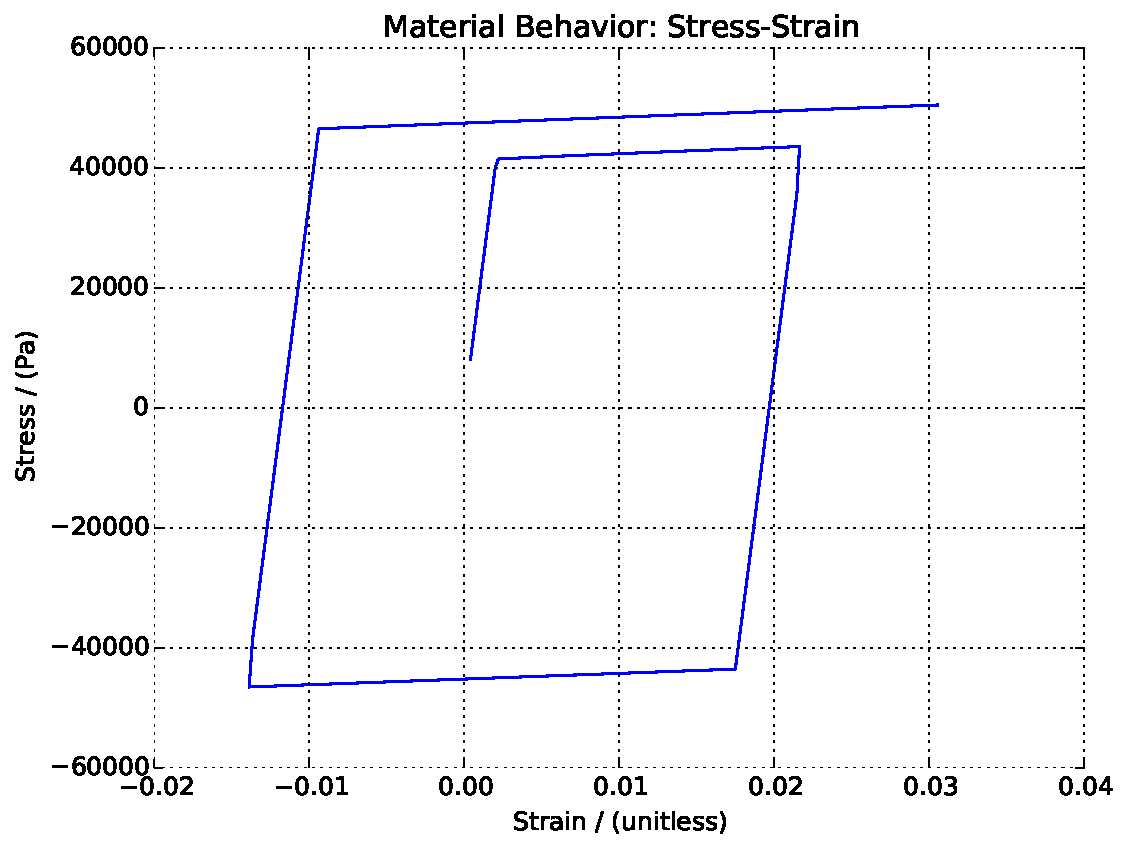
\includegraphics[width=11cm]{../fei_examples/Drucker_Prager_Associate_Flow_Solid/2pure_shear_cyclic_loading/result.pdf}
\caption{
\label{Results of Associative Drucker Prager Pure Shear Cyclic Loadin}
Results of Associative Drucker Prager Pure Shear Cyclic Loading}
\end{center}
\end{figure}

The fei files for this example are available \href{https://github.com/yuan-energy/education_examples/tree/master/fei_examples/Drucker_Prager_Associate_Flow_Solid/2pure_shear_cyclic_loading}{here}.




% %%%%%%%%%%%%%%%%%%%%%%%%%%%%%%%%%%%%%%%%%%%%%%%%%%%%%%%%%%%%%%%%%%%%%%%%%%%%
% %%%%%%%%%%%%%%%%%%%%%%%%%%%%%%%%%%%%%%%%%%%%%%%%%%%%%%%%%%%%%%%%%%%%%%%%%%%%
\newpage
\subsection{Elastic Plastic, Cam Clay Model, Various Stress Paths (To Be Added)}

% %%%%%%%%%%%%%%%%%%%%%%%%%%%%%%%%%%%%%%%%%%%%%%%%%%%%%%%%%%%%%%%%%%%%%%%%%%%%
% %%%%%%%%%%%%%%%%%%%%%%%%%%%%%%%%%%%%%%%%%%%%%%%%%%%%%%%%%%%%%%%%%%%%%%%%%%%%
% \newpage
\subsection{Elastic  Plastic, SaniSand Models, Pure Shear Solid Examples (To Be Added)}

% %%%%%%%%%%%%%%%%%%%%%%%%%%%%%%%%%%%%%%%%%%%%%%%%%%%%%%%%%%%%%%%%%%%%%%%%%%%%
% %%%%%%%%%%%%%%%%%%%%%%%%%%%%%%%%%%%%%%%%%%%%%%%%%%%%%%%%%%%%%%%%%%%%%%%%%%%%
% \newpage
\section{Stiffness Reduction and Damping Curves Modeling}

% %%%%%%%%%%%%%%%%%%%%%%%%%%%%%%%%%%%%%%%%%%%%%%%%%%%%%%%%%%%%%%%%%%%%%%%%%%%%
\subsection{Pisano Material Model (To Be Added)}


% %%%%%%%%%%%%%%%%%%%%%%%%%%%%%%%%%%%%%%%%%%%%%%%%%%%%%%%%%%%%%%%%%%%%%%%%%%%%
\newpage
\subsection{Drucker Prager with Armstrong Frederick
            Nonlinear Kinematic Hardening
            Material Model}



Model Description:

\begin{figure}[H]
\begin{center}
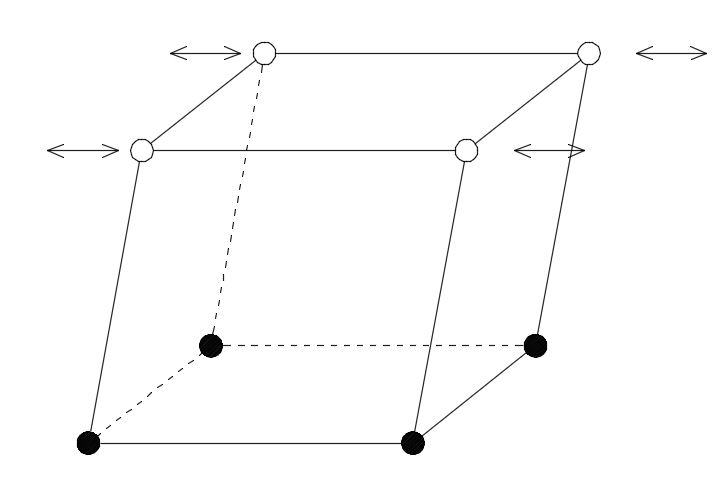
\includegraphics[width=8cm]{../Figure-files/shear_cyclic_brick.JPG}
\caption{
\label{Diagram Drucker-Prager Armstrong-Frederick Pure Shear Cyclic Loadin}
Diagram of Drucker-Prager Armstrong-Frederick Pure Shear Cyclic Loading}
\end{center}
\end{figure}

Material Response at Gauss Point:

\begin{figure}[H]
\begin{center}
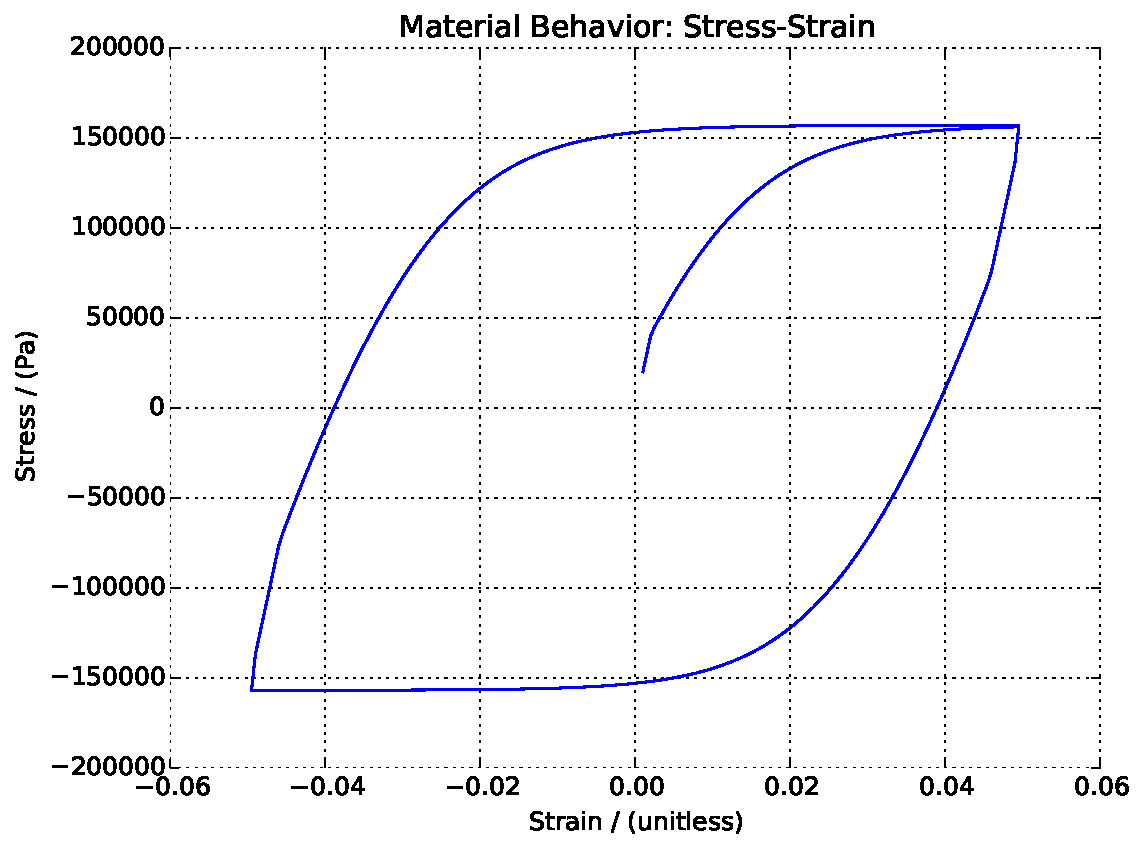
\includegraphics[width=11cm]{../fei_examples/Drucker_Prager_Armstrong_Frederick/2pure_shear_cyclic_loading/result.pdf}
\caption{
\label{Result of Drucker-Prager Armstrong-Frederick Pure Shear Cyclic Loadin}
Result of Drucker-Prager Armstrong-Frederick Pure Shear Cyclic Loading}
\end{center}
\end{figure}

The fei files for this example are available \href{https://github.com/yuan-energy/education_examples/tree/master/fei_examples/Drucker_Prager_Armstrong_Frederick/2pure_shear_cyclic_loading}{here}.







\end{document}


